\documentclass[12pt, a4paper]{article}
\usepackage[utf8]{inputenc}
\usepackage[spanish, es-tabla]{babel}
\usepackage{graphicx}
\usepackage{hyperref}
\usepackage{amsmath}
\usepackage{listings}
\usepackage{xcolor}
\usepackage[most]{tcolorbox}
\usepackage{geometry}
\usepackage{enumitem}
\usepackage{titlesec}
\usepackage{booktabs}
\usepackage{longtable}
\usepackage{array}
\usepackage{tabularx}
\usepackage{pdfpages}
\usepackage{float}
\usepackage{caption}
\usepackage{subcaption}
\usepackage{microtype}
\graphicspath{{media/}}
\geometry{margin=2.0cm}
\setlength{\parskip}{0.6em}
\setlength{\parindent}{0pt}

\titleformat{\section}{\large\bfseries}{\thesection}{1em}{}
\titleformat{\subsection}{\normalsize\bfseries}{\thesubsection}{1em}{}
\titleformat{\subsubsection}{\normalsize\bfseries\itshape}{\thesubsubsection}{1em}{}

\definecolor{cbAzul}{HTML}{1E5DA6}
\definecolor{cbVerde}{HTML}{2E7D32}
\definecolor{cbGris}{HTML}{5F6368}

\lstdefinestyle{csharp}{
    language=Java,
    morekeywords={var,string,bool,decimal,double,float,long,async,await,Task,record,
                  get,set,init,namespace,is,not,yield,base,foreach,in,out,ref,params,
                  sealed,readonly,override,virtual,abstract,partial,event,value},
    keywordstyle=\color{cbAzul}\bfseries,
    stringstyle=\color{cbVerde},
    commentstyle=\color{cbGris}\itshape,
    basicstyle=\ttfamily\footnotesize,
    columns=fullflexible,
    breaklines=true,
    keepspaces=true,
    showstringspaces=false,
    xleftmargin=1em,
    literate={á}{{\'a}}1 {é}{{\'e}}1 {í}{{\'i}}1 {ó}{{\'o}}1 {ú}{{\'u}}1
             {ñ}{{\~n}}1 {Á}{{\'A}}1 {É}{{\'E}}1 {Í}{{\'I}}1 {Ó}{{\'O}}1
             {Ú}{{\'U}}1 {Ñ}{{\~N}}1 {¿}{{?`}}1 {¡}{{!`}}1
}

\newtcblisting{csharpbox}[1][]{,
    breakable, enhanced, listing only,
    listing engine=listings,
    listing options={style=csharp,#1},
    title={\sffamily\bfseries C\#},
    coltitle=white, colbacktitle=cbAzul,
    colback=cbAzul!2!white, colframe=cbAzul!55!black,
    boxrule=0.6pt, arc=1.5mm,
    toprule=1.2pt, bottomrule=0.6pt,
    left=6pt, right=6pt, top=2pt, bottom=2pt,
    before skip=0.9em, after skip=1.1em,
}

\begin{document}
    \begin{titlepage}
        \centering
        \textbf{Universidad de La Habana \\
        Facultad de Matemática y Computación \\
        Año: 3ro\\
        Asignatura: Ingeniería de Software}\\[2cm]

        \begin{figure}[H]
            \centering
            
\includegraphics[width=0.45\textwidth]{logo.jpg}
        \end{figure}

        \vspace{1cm}

        {\LARGE \textbf{Seminario de Arquitecturas de Software:}}\\[0.5cm]

        {\large \textbf{Un Análisis Comparativo de Estilos Basados en Capas y Dominio}}

        \vspace{1.5cm}

        \textbf{Nombre de Equipo: SQLote}\\
        \begin{tabular}{ll}
            \textbf{Nombre y Apellidos} & \textbf{Pregunta} \\
            Ana Laura Oliva Avilés & 6 y 4\\
            Andriu Ferreyra Rodríguez & 3 \\
            Diana Martínez Almanza & 2 \\
            Yisell Velázquez Ochoa & 1 \\
            José Antonio Bello Cabrera & 5 \\
        \end{tabular}\\
        \href{https://github.com/AnaLauraOliva/matcom-bench-press}{https://github.com/AnaLauraOliva/matcom-bench-press}

        \vfil

        Curso: 2026-2027
    \end{titlepage}
    \tableofcontents

    \newpage
    \section[Análisis Comparativo de Comunicación y Acoplamiento]{Pregunta 1: Análisis Comparativo de Comunicación y Acoplamiento}
    \subsection{Pregunta}
    Un sistema de subastas en línea requiere que, al finalizar una subasta, se realicen múltiples acciones: notificar al ganador, procesar el pago y actualizar el inventario. En un diseño con Microservicios, un arquitecto podría optar por una coreografía de eventos (comunicación asíncrona) o una orquestación mediante un servicio mediador. En un diseño con Service-Based Architecture, estas acciones probablemente se ejecutarían dentro de un mismo servicio de dominio de grano grueso. Basado en los conceptos de connascence (connascencia) y los trade-offs de la comunicación síncrona vs. asíncrona, analice:

    \begin{itemize}
        \item ¿Cómo afecta cada enfoque (orquestación vs. coreografía en microservicios, y servicios de grano grueso en SBA) al acoplamiento dinámico entre los componentes del sistema?
        \item ¿Qué implicaciones tiene cada diseño para la tolerancia a fallos y la consistencia de los datos (ACID vs. BASE) si el servicio de pago falla justo después de que se notifica al ganador?
    \end{itemize}

    \subsection{Fundamentos: estilo arquitectónico, connascence y comunicación}

    En el diseño de sistemas distribuidos, la elección del estilo arquitectónico y del mecanismo de comunicación define el éxito o el fracaso del sistema. En un extremo se ubican los Microservicios, que buscan el máximo desacoplamiento mediante componentes pequeños y autónomos que se comunican por red, lo que ofrece una gran agilidad. Esta orientación tiene su origen en el diseño guiado por el dominio:

    “Microservicios está fuertemente inspirado por las ideas del diseño guiado por el dominio (DDD, por sus siglas en inglés), un proceso de diseño lógico para proyectos de software. Un concepto en particular del DDD, el contexto delimitado, inspiró decididamente a los microservicios. El concepto de contexto delimitado representa un estilo de desacoplamiento” (Richards \& Ford, 2020).

    En el extremo opuesto se encuentra la Service-Based Architecture (SBA), que agrupa la funcionalidad en servicios de grano grueso (dominios amplios). Al ser menos distribuida, resulta mucho más pragmática para manejar transacciones complejas, y esa misma característica le aporta una mayor fiabilidad:

    “Las arquitecturas basadas en servicios tienden a ser más fiables que otras arquitecturas distribuidas debido a la naturaleza de grano grueso de los servicios de dominio. Servicios más grandes significan menos tráfico de red hacia y entre los servicios, menos transacciones distribuidas y menos ancho de banda utilizado, aumentando por lo tanto la fiabilidad general con respecto a la red” (Richards \& Ford, 2020).

    Para comparar con rigor el grado de dependencia que cada uno de estos estilos genera entre sus componentes, resulta útil recurrir al concepto de connascence. En 1996, Meilir Page-Jones publicó What Every Programmer Should Know About Object-Oriented Design (Dorset House), obra en la que refinó las métricas de acoplamiento aferente y eferente y las reformuló para los lenguajes orientados a objetos bajo este concepto. Así definió el término:

    “Dos componentes son connascentes si un cambio en uno requeriría que el otro se modificara para mantener la corrección general del sistema” (Page-Jones, 1996, citado en Richards \& Ford, 2020).

    Más allá del estilo arquitectónico, el acoplamiento también depende de cómo se comunican los componentes, por lo que se deben evaluar los trade-offs entre la comunicación síncrona y la asíncrona. La comunicación síncrona (por ejemplo, HTTP/REST) acopla temporalmente a los componentes, ya que ambos deben estar activos en el mismo instante, lo que aumenta la fragilidad ante fallos. La comunicación asíncrona (por ejemplo, mediante eventos) elimina ese acoplamiento temporal porque el emisor no espera al receptor; sin embargo, introduce complejidad en el manejo de fallos y obliga a aceptar la consistencia eventual.

    Con estos conceptos como base, a continuación se analiza el caso de la subasta en línea.

    \subsection{Acoplamiento dinámico: orquestación, coreografía y SBA}

    El acoplamiento dinámico evalúa cómo dependen los componentes entre sí en tiempo de ejecución, midiendo qué tan fácil es realizar cambios sin propagar fallos a otros servicios.

    \textbf{Orquestación en Microservicios:} introduce un acoplamiento espacial y temporal más fuerte, típicamente mediante comunicación síncrona (HTTP/REST). El trade-off de esta comunicación es que el orquestador queda bloqueado esperando la respuesta de los servicios. Un servicio mediador controla el flujo, la secuencia y las compensaciones. Los servicios de dominio quedan acoplados al coordinador central, convirtiéndolo en un punto focal cuya lógica de secuenciación debe ser gestionada cuidadosamente. En el plano estático, esto genera connascence de nombre y de algoritmo (el orquestador conoce los nombres de los servicios y sus interfaces), mientras que en tiempo de ejecución (\textbf{acoplamiento dinámico}) introduce una fuerte \textbf{connascence de tiempo (\textit{Connascence of Timing})} —pues el orquestador y los servicios invocados deben estar disponibles simultáneamente— y \textbf{connascence de ejecución (\textit{Connascence of Execution})}, ya que el mediador impone el orden exacto de las llamadas. Si cambia la secuencia o un contrato, el orquestador debe modificarse. El acoplamiento dinámico es alto en tiempo de ejecución porque el orquestador actúa como punto de coordinación síncrona centralizado.

    \textbf{Coreografía en Microservicios (comunicación asíncrona):} representa un menor acoplamiento dinámico de ejecución en cuanto a disponibilidad temporal. Aquí el trade-off de la comunicación asíncrona es que se elimina la \textit{connascence de tiempo} (bloqueo temporal), pero se gana complejidad: los servicios deben tolerar fallos de forma autónoma y la consistencia se vuelve eventual. Los servicios (notificar ganador, procesar pago, actualizar inventario) reaccionan publicando y suscribiéndose a eventos sin conocerse directamente. La dependencia estática se limita al contrato del mensaje, permitiendo que cada servicio evolucione y se despliegue de forma autónoma. Sin embargo, en el plano dinámico aparecen \textbf{connascence de ejecución (\textit{Connascence of Execution})} y \textbf{connascence de valor (\textit{Connascence of Value})} de forma implícita: el sistema depende de que los eventos se publiquen y consuman en la secuencia correcta y con datos coherentes entre sí. Un cambio en la semántica o estructura de un evento afecta a todos los consumidores. El acoplamiento dinámico es medio-bajo, pero con mayor complejidad de observación del flujo global.

    \textbf{Servicios de grano grueso (SBA):} presentan un acoplamiento interno (estático) elevado, pero un acoplamiento dinámico (distribuido) mínimo. Toda la lógica de la subasta reside en un único servicio de dominio, por lo que las interacciones son llamadas internas en el mismo proceso, sin latencia de red ni problemas de consistencia remota. El acoplamiento dinámico entre componentes es mínimo (casi nulo a nivel de red). Solo existe acoplamiento interno de módulos dentro del servicio. El trade-off es la pérdida de independencia para desplegar y escalar cada acción por separado.

    \subsection{Tolerancia a fallos y consistencia: ACID vs. BASE}

    Si el servicio de pago falla justo después de que se notifica al ganador, el sistema debe resolver cómo deshacer o compensar la operación. La consistencia ACID busca el “todo o nada”, mientras que BASE acepta disponibilidad y consistencia eventual.

    \textbf{ACID:} conjunto de propiedades que garantiza que cada transacción se ejecute de forma fiable, incluso ante fallos del sistema o accesos concurrentes.

    \begin{itemize}
        \item \textbf{Atomicity (atomicidad):} la transacción se ejecuta por completo o no se ejecuta en absoluto.
        \item \textbf{Consistency (consistencia):} toda transacción lleva la base de datos de un estado válido a otro, sin violar sus reglas o restricciones.
        \item \textbf{Isolation (aislamiento):} las transacciones concurrentes no interfieren entre sí; cada una percibe un estado coherente.
        \item \textbf{Durability (durabilidad):} una vez confirmada (commit), la transacción persiste aunque el sistema falle justo después.
    \end{itemize}

    \textbf{BASE:} alternativa a ACID pensada para sistemas distribuidos que priorizan la disponibilidad y la tolerancia a particiones por encima de la consistencia inmediata.

    \begin{itemize}
        \item \textbf{Basically Available:} el sistema responde casi siempre, aunque a veces con datos desactualizados.
        \item \textbf{Soft state:} el estado puede cambiar con el tiempo sin una escritura explícita, mientras las réplicas convergen.
        \item \textbf{Eventual consistency:} si dejan de llegar escrituras nuevas, todas las réplicas convergen tarde o temprano al mismo valor.
    \end{itemize}

    \textbf{Coreografía (asíncrona, modelo BASE):} el sistema es altamente tolerante a fallos porque no hay un punto único de fallo central; sin embargo, la consistencia es eventual. Al fallar el pago, los servicios deben reaccionar de forma autónoma emitiendo eventos de compensación (por ejemplo, liberar el ítem y notificar al ganador que la subasta se cancela). Esto descentraliza la lógica de error, dificultando su monitoreo y depuración al estar dispersa en múltiples servicios.

    \textbf{Orquestación (modelo BASE/Sagas):} el mediador central facilita la gestión de fallos mediante transacciones de compensación (Sagas), ya que tiene visibilidad total del flujo y puede iniciar el rollback secuencial si el pago falla. El riesgo reside en que el orquestador se convierte en un cuello de botella y un punto único de fallo; si este cae, toda la transacción se detiene.

    \textbf{SBA (modelo ACID):} al ejecutarse todo dentro de un mismo servicio de dominio, es factible utilizar transacciones ACID locales para garantizar atomicidad, consistencia fuerte y rollback inmediato sobre la base de datos. No obstante, dado que el enunciado plantea que el fallo del pago ocurre \textit{después} de haber notificado al ganador, se debe tener en cuenta que un rollback de base de datos no puede deshacer un efecto secundario externo ya emitido (como un correo electrónico o notificación \textit{push}). Por ello, en SBA la notificación debe enviarse únicamente tras confirmar el commit local del pago y del inventario, o bien emitir un mensaje compensatorio de anulación si la notificación ya salió del sistema. Aun con este recaudo, la tolerancia a fallos se simplifica enormemente al evitar la complejidad de las transacciones distribuidas por red, aunque el servicio se vuelve más pesado y difícil de escalar de forma independiente.

    “La arquitectura basada en servicios preserva las transacciones ACID mejor que cualquier otra arquitectura distribuida” (Richards \& Ford, 2020).

    Si el equipo prioriza la autonomía y la escalabilidad con consistencia eventual, la coreografía es ideal; si se requiere claridad en el flujo y manejo centralizado de errores en transacciones distribuidas, la orquestación es preferible; y si la integridad transaccional inmediata es crítica y el dominio no es excesivamente grande, un servicio de grano grueso (SBA) con ACID local resulta la opción más segura.

    \section[Diseño para Elasticidad Extrema y Consistencia de Datos]{Pregunta 2: Diseño para Elasticidad Extrema y Consistencia de Datos}
    \subsection{Pregunta}
    Considere el sistema de venta de entradas para conciertos descrito en el libro (Capítulo 15). Durante el lanzamiento de entradas para un artista popular, el sistema experimenta un aumento repentino de usuarios de cientos a decenas de miles en segundos. Se le pide, como arquitecto, diseñar la solución.

    \begin{itemize}
        \item Justifique por qué una Space-Based Architecture sería una elección más adecuada que una Microservices Architecture para este escenario específico, enfocándose en las características de elasticidad y escalabilidad.
        \item Sin embargo, la Space-Based Architecture introduce el problema de las colisiones de datos en cachés replicadas. Describa cómo un arquitecto podría mitigar el riesgo de colisiones de datos en el contexto de la venta de asientos numerados, donde la consistencia es crucial. ¿Qué mecanismos o trade-offs consideraría?
    \end{itemize}

    \subsection{Contexto del problema}


    Se analiza el diseño de una plataforma de venta de entradas para conciertos en línea. Este dominio presenta una dinámica particular: el sistema opera bajo una demanda baja o moderada durante la mayor parte del tiempo, pero en el instante en que se abre la venta para un artista popular, el volumen de usuarios concurrentes se dispara de cientos a decenas de miles en cuestión de segundos (Richards \& Ford, 2020).
    \subsection{Justificación de Space-Based Architecture frente a Microservices Architecture}
    Para abordar un incremento de tráfico tan agresivo e impredecible, el estilo Space-Based Architecture (SBA) resulta más apropiado que una arquitectura de microservicios. La razón principal radica en cómo gestiona cada arquitectura el acceso a los datos y el escalado de componentes.
    \subsubsection{La eliminación del cuello de botella en la base de datos (Escalabilidad)}
    \textbf{El problema de la base de datos en Microservicios:} Si bien en microservicios cada servicio tiene su propia base de datos para garantizar la independencia del dominio (Richards \& Ford, 2020), los servicios clave que participan en la compra (como inventario de entradas, pedidos y pagos) reciben toda la carga de forma simultánea. Al escalar los microservicios horizontalmente, solo trasladamos el embudo hacia las bases de datos relacionales subyacentes. Se genera así la conocida topología en triángulo, donde la capa web y de aplicación es ancha y fácil de escalar, pero la base de datos queda en la punta como el eslabón más angosto y costoso de ampliar (Richards \& Ford, 2020). Esto produce saturación de las conexiones disponibles, contención por bloqueos en disco y caídas en cascada por tiempos de espera agotados (Ford, Richards, Sadalage \& Dehghani, 2021).

    \textbf{Procesamiento en memoria en SBA:} La arquitectura basada en el espacio soluciona esto retirando la base de datos física del flujo transaccional directo (Richards \& Ford, 2020). Las unidades de procesamiento (processing units) mantienen la lógica de negocio y los datos directamente en RAM mediante una malla de datos en memoria (in-memory data grid), implementada comúnmente con herramientas como Hazelcast, Apache Ignite o Oracle Coherence (Richards \& Ford, 2020). Las lecturas y reservas ocurren en memoria, mientras que la persistencia en disco se delega de forma asíncrona mediante bombas de datos (data pumps) y escritores de datos (data writers) (Richards \& Ford, 2020). Esto permite a SBA alcanzar una valoración de 5 estrellas en escalabilidad y rendimiento, soportando picos extremos sin degradación (Richards \& Ford, 2020).
    \subsubsection{Tiempos de respuesta ante la elasticidad (MTTS)}
    \textbf{Retraso de arranque en Microservicios:} Ante un pico súbito de demanda en segundos, levantar nuevos contenedores de microservicios toma tiempo (arranque de entornos de ejecución, conexión con el registro de servicios y configuración de pools de conexiones). Este tiempo medio de arranque (Mean Time to Start o MTTS) impide reaccionar con la rapidez necesaria y agrava la contención en la base de datos al abrir más conexiones concurrentes (Ford, Richards, Sadalage \& Dehghani, 2021).

    \textbf{Precalentamiento y replicación rápida en SBA:} SBA incluye en su middleware virtualizado un gestor de despliegue (deployment manager) que monitoriza constantemente la carga (Richards \& Ford, 2020). Dado que el inicio de una preventa tiene una hora fijada, el gestor de despliegue puede preaprovisionar (pre-warm) las unidades de procesamiento necesarias minutos antes de abrir la venta (Richards \& Ford, 2020). Además, cuando una nueva unidad de procesamiento arranca, se registra en la lista de miembros (membership list) y copia el estado de la caché desde otra instancia en memoria en menos de 100 ms, sin tocar la base de datos relacional (Richards \& Ford, 2020). Los lectores de datos (data readers) solo intervienen si se produce una caída total del clúster o para consultar datos históricos archivados (Richards \& Ford, 2020).
    \subsubsection{El alcance del quantum arquitectónico}


    Como explican Richards y Ford (2020), en SBA la base de datos no forma parte de la ecuación del quantum arquitectónico porque las unidades de procesamiento no dependen de ella de forma sincrónica. En microservicios, en cambio, la base de datos sí queda atada al quantum del servicio (Richards \& Ford, 2020), lo que limita su capacidad operativa a las restricciones físicas del motor de persistencia.
    \subsection{Mitigación del riesgo de colisiones de datos en asientos numerados}
    \subsubsection{El problema de las colisiones en cachés replicadas}
    Cuando se utiliza una caché replicada en modo activo/activo, cualquier unidad de procesamiento puede aceptar peticiones de compra. Si dos usuarios eligen la misma butaca en unidades distintas antes de que se complete la sincronización asíncrona entre ellas, ambas unidades darán la reserva por buena localmente. Al replicarse los datos, una escritura sobrescribirá a la otra, generando sobreventa (double-booking) e inconsistencias graves en el inventario (Richards \& Ford, 2020).

    Richards y Ford (2020) modelan este comportamiento mediante la siguiente fórmula:
    \begin{equation}
    \text{Tasa de colisión} = N \cdot \frac{\text{UR}^{2}}{S} \cdot \text{RL}
    \end{equation}
    donde:

    \begin{itemize}
    \item $N$ es el número de instancias de procesamiento activas.
    \item $\text{UR}$ es la tasa de actualizaciones por segundo por instancia.
    \item $S$ es el tamaño de la caché (número de asientos disponibles).
    \item $\text{RL}$ es la latencia de replicación de la malla de datos.
    \end{itemize}

    En un concierto con alta demanda, la tasa de actualización ($\text{UR}$) es enorme y el número de asientos libres ($S$) baja rápidamente a medida que se agotan las entradas. Esta combinación dispara la probabilidad de colisiones, lo que hace inviable manejar la reserva de asientos con una caché puramente replicada.
    \subsubsection{Estrategias de mitigación y trade-offs}


    Para garantizar la consistencia en la selección de asientos sin perder las ventajas de SBA, se deben aplicar las siguientes decisiones de diseño:

    \begin{enumerate}[label=\alph*)]
    \item \textbf{Caché Distribuida para el inventario de asientos (Tabla 15-1):} En lugar de usar un único modelo de caché para todo, conviene separar los datos según su necesidad de consistencia (Richards \& Ford, 2020):
        \begin{itemize}
        \item \textbf{Caché Replicada:} Para información estática y de solo lectura (ficha del concierto, mapas del estadio, tipos de precios). Al no mutar con frecuencia, ofrece máxima velocidad y disponibilidad local en cada nodo.
        \item \textbf{Caché Distribuida:} Para el mapa de asientos numerados y su estado. El inventario se mantiene centralizado en un clúster de caché en memoria externo a las unidades de procesamiento (Richards \& Ford, 2020). Como existe una única copia del dato en memoria, el bloqueo temporal de una butaca (p. ej., un lease o reserva temporal de 10 minutos para pagar) se ejecuta de forma atómica mediante operaciones de exclusión mutua (compare-and-swap), impidiendo que dos personas aparten el mismo asiento.
        \end{itemize}

    \textbf{Trade-offs:} La caché distribuida añade latencia de red en comparación con la memoria local e introduce un posible punto único de fallo (SPOF), lo que obliga a configurar réplicas en espejo (mirroring) para el clúster de caché (Richards \& Ford, 2020).
    \item \textbf{Particionamiento por sectores o gradas:} Otra alternativa viable consiste en dividir el recinto en zonas disjuntas (Platea, Tribuna Alta, Lateral). La malla de mensajería (messaging grid) se configura para enrutar las peticiones de cada sector a un grupo exclusivo de unidades de procesamiento (Richards \& Ford, 2020). Al no haber cruce de peticiones entre unidades sobre una misma butaca, se puede mantener la velocidad de la caché replicada sin riesgo de colisión.
    \item \textbf{Por qué no utilizar Near-Cache:} Richards y Ford (2020) desaconsejan específicamente el uso de near-cache (una caché local rápida respaldada por una distribuida) en este escenario. Las cachés locales frontales de cada unidad no se sincronizan entre sí, por lo que distintos nodos tendrían visiones desalineadas del inventario, mostrando butacas disponibles que en realidad ya fueron vendidas por otra unidad.
    \end{enumerate}
    \begin{table}[H]
    \centering
    \begin{tabular}{|l|p{4.5cm}|p{4.5cm}|}
                \toprule
        Criterio & Caché Replicada (Lecturas) & Caché Distribuida (Asientos) \\
                \midrule
        Objetivo principal & Rendimiento y baja latencia & Consistencia de datos \\
        Datos asignados & Información del evento y recinto & Butacas numeradas y reservas \\
        Frecuencia de cambios & Prácticamente estática & Muy alta durante la venta \\
        Riesgo de colisión & Alto con concurrencia masiva & Nulo (estado centralizado en memoria) \\
        Desventaja & Riesgo de sobreventa & Latencia de red en accesos remotos \\
                \bottomrule
    \end{tabular}
    \caption*{Tabla 1: Comparativa de modelos de caché para el sistema de entradas (basado en Richards \& Ford, 2020).}
    \end{table}

    \section[Análisis de Fallos y Resiliencia en Arquitecturas Dirigidas por Eventos]{Pregunta 3: Análisis de Fallos y Resiliencia en Arquitecturas Dirigidas por Eventos}
    \subsection{Pregunta}
    En una Event-Driven Architecture con topología de Broker, un procesador de eventos (Event Processor) falla repetidamente al procesar un tipo específico de mensaje debido a un error en los datos.

    \begin{itemize}
        \item Describa el impacto de este fallo en el flujo general del sistema y en la experiencia del usuario final, considerando que no hay un mediador central.
        \item Proponga una solución arquitectónica utilizando el Workflow Event Pattern (Patrón de Eventos de Flujo de Trabajo) descrito en el Capítulo 14. Explique detalladamente cómo este patrón mitiga el problema y qué componentes adicionales (como el workflow processor y el dashboard) serían necesarios, así como los trade-offs que introduce (p. ej., el procesamiento fuera de orden).
    \end{itemize}

    \subsection{Impacto del fallo en el flujo general y en la experiencia del usuario}
En una arquitectura dirigida por eventos (EDA) con topología de Broker, no existe ningún componente central que orqueste o supervise el proceso completo (Richards \& Ford, 2020). El sistema funciona como una carrera de relevos: cada procesador de eventos (Event Processor) recoge un mensaje, realiza su tarea y emite un nuevo evento de procesamiento a un canal o topic para que otros procesadores continúen con las siguientes etapas (Richards \& Ford, 2020).
    \subsubsection{Impacto en el funcionamiento interno del sistema}
    \textbf{Falta de visibilidad centralizada del estado global:} Como no hay un mediador que centralice y supervise el flujo completo, ningún componente tiene necesariamente conocimiento del estado de toda la transacción (Richards \& Ford, 2020). Si un procesador (por ejemplo, el de cobros) falla repetidamente al procesar un mensaje con datos incorrectos, los demás procesadores pueden continuar ejecutando sus tareas sin conocer el fallo. Esto no significa que sea imposible detectar o monitorizar estos errores, sino que la arquitectura no dispone de un mecanismo central de coordinación que identifique automáticamente cómo afecta el fallo al proceso de negocio completo.

    \textbf{Inconsistencia de datos por ejecución parcial:} Los procesadores que trabajan en paralelo a partir de eventos anteriores siguen su curso con normalidad (Richards \& Ford, 2020). Si el procesador de inventario ya descontó el artículo al recibir order-created, pero el servicio de cobro falla de forma definitiva por un error de formato, el stock queda decrementado mientras que el cobro nunca se realiza.

    \textbf{Ausencia de coordinación central para las compensaciones:} A diferencia de una arquitectura con mediador, en la topología Broker no existe un componente central que controle el estado de toda la transacción y coordine automáticamente las operaciones compensatorias (Richards \& Ford, 2020). Sin embargo, esto no significa que las compensaciones sean imposibles: pueden implementarse mediante eventos específicos de compensación a los que reaccionen los servicios participantes. El inconveniente es que cada servicio debe gestionar su propia lógica de recuperación, lo que aumenta la complejidad de coordinación. Tampoco es conveniente reenviar indiscriminadamente el evento original desde el inicio, ya que podría provocar operaciones duplicadas en los servicios que ya completaron sus tareas, si estos no implementan mecanismos de idempotencia.

    \textbf{Comportamiento de la cola:} Depende de cómo esté configurado el mecanismo de confirmación de mensajes y de las garantías proporcionadas por el broker:

    \begin{itemize}
    \item Con \textbf{Auto Acknowledge Mode}: el broker confirma automáticamente la recepción del mensaje cuando lo entrega al consumidor. Si el procesador falla después de esa confirmación, pero antes de completar el procesamiento, el mensaje puede perderse, ya que el broker lo considera entregado correctamente.
    \item Con \textbf{Client Acknowledge Mode}: el consumidor debe confirmar explícitamente que ha recibido y procesado el mensaje. Si el procesador falla antes de confirmarlo, el broker puede volver a entregarlo. Cuando se utiliza una cola FIFO con un único consumidor o con garantías estrictas de orden, los reintentos repetidos de un mensaje defectuoso pueden provocar un bloqueo de cabeza de cola (head-of-line blocking), impidiendo procesar los mensajes posteriores. Para evitarlo, se pueden configurar políticas de reintentos y mecanismos de redirección a una cola de mensajes no entregados (Dead Letter Queue o DLQ) después de alcanzar un límite de intentos (Ford, Richards, Sadalage \& Dehghani, 2021).
    \end{itemize}

    Es importante señalar que este bloqueo no ocurre necesariamente en todos los brokers ni en todas las configuraciones, ya que depende de las garantías de orden y de las políticas de consumo establecidas.

    \subsubsection{Impacto en la experiencia del usuario final}
    \textbf{Falsa confirmación inicial de éxito:} Gracias al desacoplamiento asíncrono, la aplicación suele responder al cliente casi al instante (alrededor de 25 ms mediante una semántica de tipo fire-and-forget), confirmando que la orden fue recibida (Richards \& Ford, 2020). El usuario da por hecho que su compra se procesará sin problemas.

    \textbf{El limbo transaccional:} Como el fallo ocurre más adelante en el backend y no existe un canal síncrono de respuesta que informe inmediatamente al cliente del resultado final, el usuario puede quedarse sin conocer el estado real de su operación (Richards \& Ford, 2020). Si la aplicación únicamente confirma la recepción de la orden y no dispone de mecanismos adicionales de consulta de estado o notificación asíncrona, el cliente no recibirá información sobre el error. Su pedido podría quedar sin completar ni enviar, dejándolo desinformado hasta que decida contactar al soporte técnico por su cuenta.
    \subsection{Solución propuesta: aplicación del Workflow Event Pattern}
El Workflow Event Pattern (Patrón de Eventos de Flujo de Trabajo), originado en los principios de la arquitectura reactiva, permite gestionar errores en entornos asíncronos mediante tres acciones clave: delegación, contención y reparación, asegurando que el sistema sea resiliente sin sacrificar la capacidad de respuesta (responsiveness) (Richards \& Ford, 2020).
    \subsubsection{Mecanismo de mitigación y flujo de 6 pasos}
En lugar de permitir que un mensaje corrupto bloquee la cola mediante reintentos indefinidos, el flujo se organiza en los seis pasos descritos por Richards y Ford (2020):

    \begin{enumerate}
    \item El emisor envía el mensaje de forma asíncrona a la cola principal.
    \item El procesador de eventos detecta un error en los datos (por ejemplo, una excepción NumberFormatException provocada por recibir ``8756 SHARES'' en un campo numérico) (Richards \& Ford, 2020).
    \item El procesador no intenta solucionar el fallo en su propio hilo: delega el mensaje de inmediato a un canal secundario de errores junto con el detalle de la excepción. Solo después de recibir la confirmación de que el mensaje ha sido almacenado correctamente en dicho canal, confirma la recepción en la cola original (client acknowledge) y pasa al siguiente mensaje. Si no se consigue almacenar el mensaje en el canal secundario, no debe confirmarse el original, permitiendo que el broker vuelva a entregarlo. De esta forma se evita perder mensajes durante la transferencia y se mantiene el rendimiento general del sistema (Richards \& Ford, 2020).
    \item El componente especializado Workflow Processor recibe el mensaje anómalo e intenta corregirlo.
    \item Una vez subsanado, el Workflow Processor reenvía el mensaje reparado a la cola original.
    \item El procesador de eventos principal recibe el mensaje limpio y completa la transacción con éxito.
    \end{enumerate}
    \subsubsection{Componentes necesarios en la solución}
    \begin{itemize}
    \item \textbf{Canal de eventos de error:} Cola persistente dedicada que traslada los mensajes fallidos desde los procesadores hacia el componente de reparación.
    \item \textbf{Workflow Processor (Procesador de flujo de trabajo):} Servicio encargado de analizar la causa del error. Puede aplicar correcciones programáticas mediante reglas directas (como limpiar la palabra ``SHARES'' para dejar únicamente el valor numérico 8756) o algoritmos de detección de anomalías (Richards \& Ford, 2020).
    \item \textbf{Dashboard (Tablero de control):} Panel visual interactivo al que se envían los mensajes que el procesador no pudo corregir de forma automática (Richards \& Ford, 2020). Un operador de soporte revisa los datos en pantalla, corrige manualmente los campos defectuosos y reinyecta el mensaje a la cola original utilizando la cabecera de transporte reply-to (Richards \& Ford, 2020).
    \item \textbf{Dead Letter Queue (DLQ):} Cola destinada a conservar los mensajes que no han podido procesarse correctamente después de agotar los reintentos establecidos o que han sido identificados como irrecuperables (Ford, Richards, Sadalage \& Dehghani, 2021). Debe distinguirse del canal de eventos de error utilizado por el Workflow Event Pattern: este último permite trasladar los mensajes defectuosos al Workflow Processor y al Dashboard para intentar repararlos, mientras que la DLQ conserva aquellos mensajes que finalmente no pueden recuperarse. De esta forma, los mensajes problemáticos quedan aislados para su posterior investigación sin bloquear indefinidamente el procesamiento normal.
    \end{itemize}
    
    \textbf{Idempotencia y prevención de mensajes duplicados:} Debido a que el broker puede entregar un mismo mensaje más de una vez, especialmente cuando ocurren fallos durante su procesamiento o confirmación, los consumidores deben implementar mecanismos de idempotencia. Para ello, cada evento debe contar con un identificador único que permita reconocer si ya fue procesado anteriormente. El consumidor puede mantener un registro de los identificadores de los eventos procesados y comprobarlo antes de ejecutar nuevamente la operación. Esta comprobación y la actualización de los datos de negocio deben protegerse mediante una misma transacción local, apoyándose también en restricciones de unicidad en la base de datos. Así se evita que los reintentos o la reinyección de mensajes reparados provoquen operaciones duplicadas o alteraciones incorrectas del estado del sistema.

    \subsubsection{Trade-offs y contrapartidas del patrón}
    \textbf{Procesamiento fuera de orden (Out-of-sequence processing):} Es la principal desventaja del patrón (Richards \& Ford, 2020). Mientras el mensaje con error se desvía para ser reparado, los mensajes que llegaron después se siguen procesando con normalidad. Cuando el mensaje corregido vuelve a la cola, entra con un orden temporal alterado respecto a los sucesos posteriores.

    \textbf{Estrategia de mitigación para el orden:} Si el dominio exige un orden estricto (como en transacciones financieras donde una venta debe ocurrir antes de una compra en una misma cuenta), el servicio debe capturar el identificador de la entidad afectada, por ejemplo, el identificador de la cuenta, y garantizar que todos los mensajes correspondientes a ella se procesen secuencialmente. Para ello, puede utilizarse una cola FIFO o un mecanismo de particionamiento que mantenga los mensajes de una misma cuenta dentro de un único flujo ordenado. Los mensajes posteriores de esa cuenta deben permanecer temporalmente pendientes hasta que el mensaje defectuoso sea reparado y procesado correctamente. Mientras tanto, los mensajes correspondientes a otras cuentas pueden continuar procesándose con normalidad. También pueden utilizarse números de secuencia o versiones para detectar mensajes que llegan fuera de orden (Richards \& Ford, 2020).

    \textbf{Mayor complejidad en infraestructura:} Supone implementar y mantener colas adicionales, componentes dedicados de reparación y la interfaz web del dashboard, lo que aumenta el esfuerzo de despliegue y mantenimiento (Richards \& Ford, 2020).
    \section[El Dilema de la Granularidad y el Acoplamiento en Microservicios]{Pregunta 4: El Dilema de la Granularidad y el Acoplamiento en Microservicios}

    \subsection{Pregunta}

    El Dilema de la Granularidad y el Acoplamiento en Microservicios: Un equipo de desarrollo está migrando un sistema monolítico de gestión de recursos humanos a Microservicios. Inicialmente, crean servicios muy pequeños para cada entidad (Empleado, Departamento, Nómina, Beneficios). Pronto descubren que completar una operación simple, como contratar a un nuevo empleado, requiere una compleja coreografía de llamadas síncronas entre casi todos los servicios, lo que resulta en un alto acoplamiento y una fragilidad similar a la del monolito original.

    Basado en los principios de bounded context y las guías de granularidad del Capítulo 17, ¿cuál fue el error fundamental en el diseño de los servicios?

    Proponga una nueva estrategia de descomposición. ¿Cómo aplicaría los conceptos de propósito, transacciones y coreografía para redefinir los límites de los servicios y reducir el acoplamiento? Proporcione un ejemplo de cómo agruparía los servicios para la operación de “contratación”.

    \subsection{Error fundamental en el diseño de los servicios}

    Teniendo en cuenta la división de servicios actual, contratar a un nuevo empleado implicaría una cadena de llamadas síncronas entre los cuatro microservicios, donde cada uno tendría que solicitar información o ejecutar operaciones en los demás para completar el proceso. Para ver este flujo con más detalle, veamos un ejemplo.

    Luego de implementar la nueva arquitectura, el departamento de Recursos Humanos de la empresa necesita contratar a un nuevo empleado, llamémoslo Juan Pérez, quien ocupará el cargo de desarrollador de software en el Departamento de Desarrollo. Para completar su contratación, el sistema debe registrar sus datos personales, verificar el departamento al que será asignado, establecer su salario y determinar los beneficios que le corresponden.

    Cuando el responsable de Recursos Humanos introduce la información y confirma la contratación se produce la siguiente secuencia hipotética (figura 4.1): el servicio Empleado recibe la solicitud de contratación y registra los datos personales del nuevo empleado; sin embargo, para continuar necesita verificar que el departamento solicitado existe y confirmar la asignación antes de continuar con el proceso, de ahí que llame síncronamente al servicio Departamento.

    \begin{figure}[H]

        \centering

        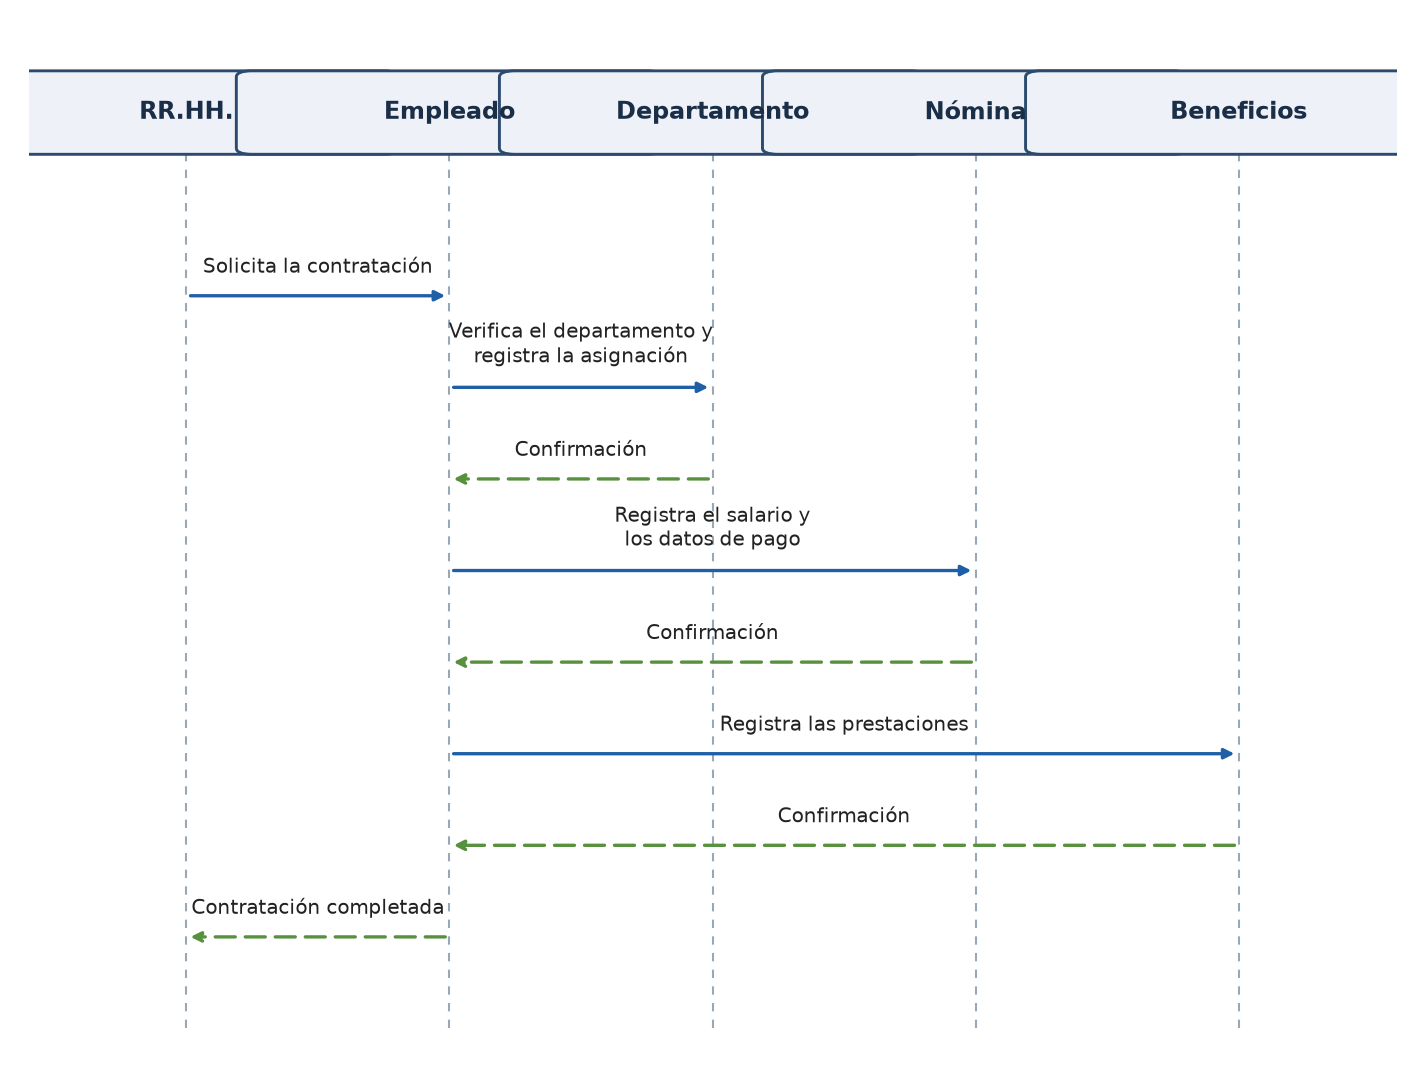
\includegraphics[width=0.75\textwidth]{figura-4-1-secuencia-contratacion.png}

        \caption*{Figura 4.1: Secuencia hipotética de la contratación mediante llamadas síncronas entre los servicios.}

    \end{figure}

    El servicio Departamento recibe la llamada del servicio Empleado, verifica la existencia del departamento de Desarrollo y registra la asignación de Juan Pérez y, posteriormente, le devuelve la respuesta al servicio Empleado con el resultado de la operación. Una vez completada la asignación, el servicio Empleado necesita garantizar que el trabajador quede registrado en el sistema de pagos y que su salario haya sido configurado antes de considerar completada su incorporación administrativa, para ello llama síncronamente al servicio Nómina, que registra los datos salariales del empleado y configura la información necesaria para procesar sus pagos y, entonces, devuelve la confirmación al servicio Empleado.

    Una vez recibida la confirmación, el servicio Empleado llama síncronamente al servicio Beneficios, ya que necesita conocer qué prestaciones le corresponden al trabajador y confirmar que estas han sido asignadas como parte de su contratación. Beneficios, entonces, consulta las políticas de beneficios aplicables al nuevo empleado, registra las prestaciones correspondientes y devuelve el resultado de la operación, que es recibido por Empleado y, tras comprobar que todas las operaciones finalizaron correctamente, informa al responsable de Recursos Humanos que la contratación ha sido completada.

    Richards \& Ford (2020) plantean que a los arquitectos les cuesta encontrar la granularidad correcta para los servicios en los microservicios, y que a menudo cometen el error de hacer sus servicios demasiado pequeños, como es el caso, lo que los obliga a construir enlaces de comunicación entre los servicios para realizar un trabajo útil, como bien se puede apreciar en el ejemplo de contratación.

    Los límites de los servicios en los microservicios tienen como propósito capturar un dominio o flujo de trabajo, dándose casos en los que esos límites naturales pueden ser grandes debido a que algunos procesos de negocio están más acoplados que otros (Richards \& Ford, 2020).

    Esta división en Empleado, Departamento, Nómina y Beneficios, para el caso descrito, provoca que un servicio (Empleado) necesite que el resto de los servicios esté disponible para completar la contratación; cada llamada síncrona aumenta el tiempo de respuesta de la operación y, si uno de los servicios falla (por ejemplo, el de Beneficios) después de completar el registro del empleado y configurarle la nómina, el sistema queda en un estado parcialmente completado y se necesita gestionar errores, compensaciones y posibles inconsistencias entre servicios.

    Los servicios se dividieron por entidades en lugar de por flujos de trabajo o por dominios, como sugiere la definición de contextos limitados (Richards \& Ford, 2020), provocando una granularidad extremadamente fina y distribuyendo una operación de negocio que debería tener mayor cohesión entre múltiples servicios.

    \subsection{Nueva estrategia de descomposición}

    Richards \& Ford (2020) definen algunas directrices que los arquitectos pueden utilizar para ayudar a encontrar los límites apropiados, entre ellas:

    \begin{itemize}
        \item \textbf{Propósito:} Idealmente, cada microservicio debería ser extremadamente cohesivo desde el punto de vista funcional, contribuyendo con un comportamiento significativo en beneficio de la aplicación general.
        \item \textbf{Transacciones:} Los contextos delimitados son flujos de trabajo de negocio, y a menudo las entidades que necesitan cooperar en una transacción muestran a los arquitectos un buen límite de servicio.
        \item \textbf{Coreografía:} Si se construye un conjunto de servicios que ofrecen un excelente aislamiento del dominio pero requieren una comunicación extensa para funcionar, se puede considerar volver a agrupar estos servicios en un servicio más grande para evitar la sobrecarga de comunicación.
    \end{itemize}

    Además, mencionan que la única manera de asegurar un buen diseño de servicios es la iteración.

    Iteremos y tengamos en cuenta el ejemplo de contratación para obtener una nueva división: aplicando la directriz de propósito, podemos unir Departamento y Empleado en un único servicio, debido a que son conceptos estrechamente vinculados; a este nuevo servicio lo llamaremos Personal y se encargará de registrar al empleado y ubicarlo en un departamento. No es aconsejable unir Nómina y Beneficios por ahora, ya que no se conocen con exactitud las reglas de negocio de cada una; por ello las mantendremos separadas y haremos que Personal emita un evento EmpleadoContratado que consumirán estos dos servicios de forma asíncrona y con el que Nómina registrará al empleado y Beneficios lo inscribirá. Personal ya cumple con la directriz de transacción y, si bien los arquitectos recomiendan no realizar transacciones entre servicios, algunas son inevitables; por ello dejaremos así la división. Además, como al contratar la comunicación puede hacerse de forma asíncrona y no es muy extensa, entonces la directriz de la coreografía también se cumple.

    Cuando se contrata un nuevo empleado, Recursos Humanos solicita la contratación, la petición entra a Personal; este comprueba que el departamento existe, crea al empleado y lo asigna a su departamento en una sola transacción local, para después publicar el evento EmpleadoContratado con los datos que los demás necesitan: id, nombre, cargo, salario base y fecha de ingreso. Nómina reacciona a ese evento, registra al empleado con su salario y fecha de inicio. Beneficios también reacciona e inscribe al empleado, digamos que en el plan básico.

    \subsection{Ilustración del flujo con código: el patrón Anthology Saga}

    Ilustremos este flujo con código. Usaremos el llamado patrón Anthology Saga (Ford, Richards, Sadalage \& Dehghani, 2021). Este patrón se caracteriza por usar comunicación asíncrona, consistencia eventual y coordinación coreográfica. Utiliza colas de mensajes para enviar mensajes asíncronos a otros servicios de dominio sin necesidad de orquestación.

    Antes de implementar los servicios, establezcamos el contrato del evento que permitirá comunicar la contratación:

    \begin{csharpbox}
public record EmpleadoContratado(
    Guid SagaId,
    Guid EmpleadoId,
    string Nombre,
    string Cargo,
    decimal SalarioBase,
    DateTime FechaIngreso
);
    \end{csharpbox}

    Nótese que el evento incluye SagaId: como el patrón Anthology Saga carece de un orquestador, no existe un coordinador que transporte el estado del flujo, de modo que este identificador debe viajar con cada mensaje de la Saga para que todos los participantes se refieran a la misma transacción distribuida. Además, la carga del evento lleva los datos que Nómina y Beneficios necesitan (id, nombre, cargo, salario base y fecha de ingreso), de forma que ningún consumidor tenga que volver a consultar a Personal: los datos necesarios viajan con el evento, tal como sugiere la técnica de delegación para evitar la propiedad conjunta de tablas (Ford, Richards, Sadalage \& Dehghani, 2021).

    Ahora definamos el servicio Personal. Comenzaremos con las entidades que administra el servicio:

    \begin{csharpbox}
public class Empleado
{
    public Guid Id { get; private set; }
    public string Nombre { get; private set; }
    public string Cargo { get; private set; }
    public decimal SalarioBase { get; private set; }
    public DateTime FechaIngreso { get; private set; }

    private Empleado() { }

    public Empleado(
        string nombre,
        string cargo,
        decimal salarioBase,
        DateTime fechaIngreso)
    {
        Id = Guid.NewGuid();
        Nombre = nombre;
        Cargo = cargo;
        SalarioBase = salarioBase;
        FechaIngreso = fechaIngreso;
    }
}

public class AsignacionDepartamento
{
    public Guid EmpleadoId { get; private set; }
    public Guid DepartamentoId { get; private set; }

    private AsignacionDepartamento() { }

    public AsignacionDepartamento(
        Guid empleadoId,
        Guid departamentoId)
    {
        EmpleadoId = empleadoId;
        DepartamentoId = departamentoId;
    }
}
    \end{csharpbox}

    Recursos Humanos envía una solicitud con los datos necesarios para registrar al empleado:

    \begin{csharpbox}
public record SolicitudContratacion(
    string Nombre,
    string Cargo,
    decimal SalarioBase,
    DateTime FechaIngreso,
    Guid DepartamentoId
);
    \end{csharpbox}

    El caso de uso coordina la validación del departamento, la creación del empleado y su asignación. Cuando los datos de entrada son inválidos, es preferible lanzar una excepción de dominio expresiva en lugar de una Exception genérica:

    \begin{csharpbox}
public class DepartamentoInexistenteException : Exception
{
    public DepartamentoInexistenteException(Guid departamentoId)
        : base($"El departamento {departamentoId} no existe.")
    {
    }
}
    \end{csharpbox}

    Personal, además, es el responsable de iniciar el registro de la Saga. Para que ese registro pueda actualizarse de forma idempotente y no dependa de que cada consumidor mire campos públicos, llevamos las transiciones al interior de la propia entidad (máquina de estados de la Saga):

    \begin{csharpbox}
public class EstadoContratacion
{
    public Guid SagaId { get; private set; }
    public Guid EmpleadoId { get; private set; }

    public bool NominaCompletada { get; private set; }
    public bool BeneficiosCompletados { get; private set; }
    public bool Cancelada { get; private set; }

    public bool Finalizada =>
        NominaCompletada && BeneficiosCompletados && !Cancelada;

    private EstadoContratacion() { }

    public EstadoContratacion(
        Guid sagaId,
        Guid empleadoId)
    {
        SagaId = sagaId;
        EmpleadoId = empleadoId;
    }

    // Devuelven true solo la primera vez; los reintentos
    // (eventos duplicados del intermediario) las ignoran.
    public bool MarcarNominaCompletada()
    {
        if (NominaCompletada || Cancelada)
            return false;
        NominaCompletada = true;
        return true;
    }

    public bool MarcarBeneficiosCompletados()
    {
        if (BeneficiosCompletados || Cancelada)
            return false;
        BeneficiosCompletados = true;
        return true;
    }

    public void Cancelar() => Cancelada = true;
}
    \end{csharpbox}

    El caso de uso de contratación queda así:

    \begin{csharpbox}
public class ContratarEmpleadoUseCase
{
    private readonly IPersonalRepository _repository;
    private readonly IEventPublisher _publisher;

    public ContratarEmpleadoUseCase(
        IPersonalRepository repository,
        IEventPublisher publisher)
    {
        _repository = repository;
        _publisher = publisher;
    }

    public async Task<Guid> Ejecutar(
        SolicitudContratacion solicitud)
    {
        // 1. Comprobar que el departamento existe.
        var departamento = await _repository
            .ObtenerDepartamento(solicitud.DepartamentoId);

        if (departamento is null)
            throw new DepartamentoInexistenteException(
                solicitud.DepartamentoId);

        // 2. Iniciar la Saga con un único SagaId; todos los
        //    participantes de este flujo lo compartirán.
        var sagaId = Guid.NewGuid();

        // 3. Crear al empleado y su asignación departamental.
        var empleado = new Empleado(
            solicitud.Nombre,
            solicitud.Cargo,
            solicitud.SalarioBase,
            solicitud.FechaIngreso
        );

        var asignacion = new AsignacionDepartamento(
            empleado.Id,
            departamento.Id
        );

        var saga = new EstadoContratacion(sagaId, empleado.Id);

        var evento = new EmpleadoContratado(
            sagaId,
            empleado.Id,
            empleado.Nombre,
            empleado.Cargo,
            empleado.SalarioBase,
            empleado.FechaIngreso
        );

        // 4. Una única transacción local confirma al empleado,
        //    su asignación, el estado de la Saga y el evento
        //    en la bandeja de salida.
        await _repository.EjecutarTransaccion(async () =>
        {
            await _repository.GuardarEmpleado(empleado);
            await _repository.GuardarAsignacion(asignacion);
            await _repository.GuardarEstadoSaga(saga);
            await _repository.GuardarMensajePendiente(evento);
        });

        // 5. Publicar el evento al intermediario de mensajería y
        //    marcar el mensaje como enviado en la bandeja de
        //    salida, para que el despachador no lo reenvíe. Si la
        //    publicación falla, el mensaje queda pendiente y el
        //    despachador lo reenvía más tarde; si el marcado
        //    falla tras una publicación exitosa, el reenvío
        //    duplica el evento, lo cual no daña: los
        //    consumidores aplican idempotencia.
        await _publisher.Publicar(evento);
        await _repository.MarcarMensajeEnviado(evento);

        return empleado.Id;
    }
}
    \end{csharpbox}

    En el código anterior confluyen cuatro decisiones. Primero, la comprobación del departamento se realiza antes de registrar la contratación y falla con una excepción de dominio. Segundo, la creación del empleado, su asignación y el estado inicial de la Saga se confirman conjuntamente en una única transacción local. Tercero, el evento se guarda también en esa transacción, en una bandeja de salida (outbox): así se evita el hueco clásico de publicar después de confirmar, donde un fallo entre el commit y la publicación deja un empleado registrado sin que Nómina ni Beneficios se enteren nunca. Cuarto, tras publicar el evento se lo marca como enviado en la bandeja de salida; si la publicación falla, el mensaje queda pendiente y un despachador periódico lo reenvía, y si el marcado falla después de una publicación exitosa, el reenvío duplica el evento, lo cual no daña, pues los consumidores aplican idempotencia. Lo que nunca debe ocurrir es un mensaje guardado en la bandeja de salida que se publique sin quedar registrado como enviado: el despachador lo reenviaría indefinidamente. Los suscriptores de Nómina y Beneficios deben configurarse como suscriptores duraderos, de manera que reciban el mensaje apenas vuelvan a estar disponibles (Ford, Richards, Sadalage \& Dehghani, 2021).

    Nómina recibe el evento y ejecuta su propia transacción local para registrar al empleado. Como los intermediarios de mensajería garantizan una entrega de al menos una vez, los eventos pueden llegar duplicados: el consumidor comprueba dentro de su transacción, y no antes, para resultar idempotente incluso ante entregas concurrentes, y siempre emite la confirmación, presente o no el registro en esta entrega, por si la anterior se hubiera perdido:

    \begin{csharpbox}
public class NominaEmpleadoContratadoConsumer
{
    private readonly INominaRepository _repository;
    private readonly IEventPublisher _publisher;

    public NominaEmpleadoContratadoConsumer(
        INominaRepository repository,
        IEventPublisher publisher)
    {
        _repository = repository;
        _publisher = publisher;
    }

    public async Task Consumir(EmpleadoContratado evento)
    {
        // La política de reintentos del consumidor (no mostrada)
        // rodea a este método: solo cuando los reintentos se
        // agotan, la excepción alcanza el bloque catch.
        try
        {
            // Idempotencia y compensación: el evento puede llegar
            // duplicado y un evento de fallo puede haberse
            // anticipado. Si existe cualquier registro del
            // empleado, activo o ya cancelado, no se vuelve a
            // registrar: la cancelación, presente o futura,
            // prevalece porque ambos caminos escriben la misma
            // fila claveada por EmpleadoId, sobre la que el
            // repositorio serializa las transacciones.
            await _repository.EjecutarTransaccion(async () =>
            {
                if (await _repository.RegistroNominaExiste(evento.EmpleadoId))
                    return;

                var empleado = new EmpleadoNomina(
                    evento.EmpleadoId,
                    evento.SalarioBase,
                    evento.FechaIngreso
                );

                await _repository.RegistrarEmpleado(empleado);
            });

            // Se registre o no el empleado en esta entrega, la
            // confirmación se emite: si el registro ya existía,
            // puede que la confirmación anterior se hubiera
            // perdido y la Saga quedaría estancada. No importa si
            // el registro está cancelado: el seguimiento ignora
            // las confirmaciones de sagas canceladas.
            await PublicarConfirmacion(evento);
        }
        catch (Exception)
        {
            // Agotados los reintentos, notificamos el fallo de la
            // Saga (ContratacionFallida se define más adelante)
            // para que todos los participantes compensen. El
            // mensaje se acusa como procesado: el intermediario
            // no debe reenviarlo una vez compensada la operación.
            await _publisher.Publicar(
                new ContratacionFallida(
                    evento.SagaId,
                    evento.EmpleadoId,
                    "Nómina no pudo registrar al empleado."));
        }
    }

    private Task PublicarConfirmacion(EmpleadoContratado evento) =>
        _publisher.Publicar(
            new EmpleadoRegistradoEnNomina(
                evento.SagaId,
                evento.EmpleadoId
            )
        );
}
    \end{csharpbox}

    Tras completar su operación, Nómina publica un evento de confirmación.

    \begin{csharpbox}
public record EmpleadoRegistradoEnNomina(
    Guid SagaId,
    Guid EmpleadoId
);
    \end{csharpbox}

    Este evento hace posible identificar que la participación de Nómina en la Saga ha concluido satisfactoriamente.

    Por su parte, Beneficios también recibe EmpleadoContratado, pero ejecuta una operación diferente: inscribir al empleado en el plan básico. Renombrado el consumidor (cada servicio tiene el suyo) y aplicado el mismo tratamiento idempotente y de fallos que en Nómina:

    \begin{csharpbox}
public class InscripcionBeneficio
{
    public Guid EmpleadoId { get; private set; }
    public string Plan { get; private set; }
    public DateTime FechaInscripcion { get; private set; }

    private InscripcionBeneficio() { }

    public InscripcionBeneficio(Guid empleadoId)
    {
        EmpleadoId = empleadoId;
        Plan = "Básico";
        FechaInscripcion = DateTime.UtcNow;
    }
}

public class BeneficiosEmpleadoContratadoConsumer
{
    private readonly IBeneficiosRepository _repository;
    private readonly IEventPublisher _publisher;

    public BeneficiosEmpleadoContratadoConsumer(
        IBeneficiosRepository repository,
        IEventPublisher publisher)
    {
        _repository = repository;
        _publisher = publisher;
    }

    public async Task Consumir(EmpleadoContratado evento)
    {
        // La política de reintentos del consumidor (no mostrada)
        // rodea a este método, igual que en Nómina.
        try
        {
            // Idempotencia y compensación, igual que en Nómina:
            // si existe cualquier inscripción, activa o ya
            // cancelada, no se vuelve a inscribir, y una
            // cancelación anticipada prevalece porque ambos
            // caminos escriben la misma fila claveada por
            // EmpleadoId.
            await _repository.EjecutarTransaccion(async () =>
            {
                if (await _repository.InscripcionExiste(evento.EmpleadoId))
                    return;

                var inscripcion = new InscripcionBeneficio(
                    evento.EmpleadoId
                );

                await _repository.Inscribir(inscripcion);
            });

            // Confirmación siempre emitida, presente o no la
            // inscripción en esta entrega, por si la anterior
            // se hubiera perdido.
            await PublicarConfirmacion(evento);
        }
        catch (Exception)
        {
            // Agotados los reintentos, notificamos el fallo de la
            // Saga para que todos los participantes compensen.
            await _publisher.Publicar(
                new ContratacionFallida(
                    evento.SagaId,
                    evento.EmpleadoId,
                    "Beneficios no pudo inscribir al empleado."));
        }
    }

    private Task PublicarConfirmacion(EmpleadoContratado evento) =>
        _publisher.Publicar(
            new EmpleadoInscritoEnBeneficios(
                evento.SagaId,
                evento.EmpleadoId
            )
        );
}
    \end{csharpbox}

    También tiene su evento de confirmación que informa que Beneficios ha completado su participación en el proceso de contratación:

    \begin{csharpbox}
public record EmpleadoInscritoEnBeneficios(
    Guid SagaId,
    Guid EmpleadoId
);
    \end{csharpbox}

    Hasta el momento tenemos los eventos que permiten comunicar las operaciones realizadas por cada participante.

    Para conocer cuándo termina el proceso completo, mantenemos el registro del estado de la Saga que Personal inicializa al publicar EmpleadoContratado. El seguimiento solo observa los eventos de confirmación y usa las transiciones idempotentes de la entidad; como Nómina y Beneficios confirman de forma independiente, sus mensajes pueden procesarse a la vez, de modo que cada transición se ejecuta dentro de una transacción que serializa el acceso a la fila de la Saga:

    \begin{csharpbox}
public class SeguimientoContratacionConsumer
{
    private readonly ISagaRepository _repository;

    public SeguimientoContratacionConsumer(
        ISagaRepository repository)
    {
        _repository = repository;
    }

    public async Task Consumir(
        EmpleadoRegistradoEnNomina evento)
    {
        // La lectura, la transición y la escritura ocurren dentro
        // de una única transacción sobre la fila de la Saga: dos
        // confirmaciones concurrentes o duplicadas no pueden leer
        // la misma versión y registrar la marca dos veces.
        await _repository.EjecutarTransaccion(async () =>
        {
            var saga = await _repository.Obtener(evento.SagaId);

            // Si la Saga no existe o la marca ya se registró,
            // el evento se ignora.
            if (saga is null || !saga.MarcarNominaCompletada())
                return;

            await _repository.Actualizar(saga);
        });
    }

    public async Task Consumir(
        EmpleadoInscritoEnBeneficios evento)
    {
        await _repository.EjecutarTransaccion(async () =>
        {
            var saga = await _repository.Obtener(evento.SagaId);

            if (saga is null || !saga.MarcarBeneficiosCompletados())
                return;

            await _repository.Actualizar(saga);
        });
    }
}
    \end{csharpbox}

    Finalmente, queda coordinar los errores. En el patrón Anthology Saga no hay orquestador que centralice el manejo de fallos: cada servicio mantiene su propia integridad transaccional y debe incluir sus propias estrategias de coordinación, incluidas las transacciones compensatorias (Ford, Richards, Sadalage \& Dehghani, 2021). Definimos entonces un evento común de fallo, el que publica Nómina desde el bloque catch de su consumidor cuando, tras agotar los reintentos, no logra completar su operación:

    \begin{csharpbox}
public record ContratacionFallida(
    Guid SagaId,
    Guid EmpleadoId,
    string Motivo
);
    \end{csharpbox}

    Un método adicional en SeguimientoContratacionConsumer cierra la Saga al ocurrir el fallo:

    \begin{csharpbox}
public async Task Consumir(ContratacionFallida evento)
{
    // Misma serialización transaccional que las confirmaciones:
    // un fallo y una confirmación pueden cruzarse en el aire.
    await _repository.EjecutarTransaccion(async () =>
    {
        var saga = await _repository.Obtener(evento.SagaId);

        // Si la Saga no existe, ya se compensó o ya finalizó,
        // el evento se ignora: no se cancela una contratación
        // que sí llegó a completarse.
        if (saga is null || saga.Cancelada || saga.Finalizada)
            return;

        saga.Cancelar();
        await _repository.Actualizar(saga);
    });
}
    \end{csharpbox}

    Todos los participantes se suscriben a ContratacionFallida y ejecutan su propia transacción compensatoria local. Por ejemplo, Nómina (el consumidor de Beneficios es simétrico: anticipa o ejecuta la cancelación de la inscripción sobre su propia fila claveada):

    \begin{csharpbox}
public class NominaContratacionFallidaConsumer
{
    private readonly INominaRepository _repository;

    public NominaContratacionFallidaConsumer(
        INominaRepository repository)
    {
        _repository = repository;
    }

    public async Task Consumir(ContratacionFallida evento)
    {
        // Transacción compensatoria local. RegistrarCancelacion
        // Nomina cubre ambos órdenes de llegada: si el registro
        // existe, lo marca como cancelado; si no existe aún,
        // inserta una fila cancelada que anticipa la cancelación,
        // de modo que un registro posterior no llegue a
        // ejecutarse. Ambos caminos (cancelar y registrar)
        // escriben la misma fila claveada por EmpleadoId, sobre
        // la que el repositorio serializa las transacciones: no
        // pueden cruzarse. Se conserva el historial para que la
        // compensación sea auditable; nada se borra físicamente.
        await _repository.EjecutarTransaccion(async () =>
        {
            await _repository.RegistrarCancelacionNomina(
                evento.EmpleadoId);
        });
    }
}
    \end{csharpbox}

    El iniciador no queda exento: Personal también debe compensar su propia transacción local anulando al empleado y su asignación departamental; de lo contrario, la compensación de los demás participantes dejaría registrado un empleado cuya contratación fracasó:

    \begin{csharpbox}
public class PersonalContratacionFallidaConsumer
{
    private readonly IPersonalRepository _repository;

    public PersonalContratacionFallidaConsumer(
        IPersonalRepository repository)
    {
        _repository = repository;
    }

    public async Task Consumir(ContratacionFallida evento)
    {
        // Transacción compensatoria local: se anulan al empleado
        // y su asignación en una única transacción, con la misma
        // serialización que el registro original. Como en los
        // demás participantes, se conserva el historial para que
        // la compensación sea auditable.
        await _repository.EjecutarTransaccion(async () =>
        {
            if (await _repository.EmpleadoExiste(evento.EmpleadoId))
            {
                await _repository.AnularEmpleado(evento.EmpleadoId);
            }
        });
    }
}
    \end{csharpbox}

    Observemos dos detalles de estas compensaciones. Primero, son idempotentes y tolerantes al reordenamiento: cada participante revierte, dentro de una única transacción, lo que llegó a ejecutar, y si el evento de fallo se anticipa a EmpleadoContratado, la cancelación se anticipa con él: la fila cancelada que deja impide que el registro o la inscripción lleguen a ejecutarse cuando el evento original arribe tarde, porque cancelación y registro disputan la misma fila y el repositorio serializa ese acceso. Segundo, SeguimientoContratacionConsumer ignora los eventos de fallo que arriban cuando la Saga ya finalizó, de manera que no se compensa una contratación que sí se completó.

    Con este cierre, la declaración Cancelada del estado de la Saga evita que un evento de confirmación llegue tarde y registre progreso sobre una transacción ya compensada. La estrategia de fallo se apoya, además, en los mecanismos del patrón basado en eventos para consistencia eventual: los servicios que reaccionan al evento deben configurarse como suscriptores duraderos para no perder nada si están caídos, el intermediario reintenta la entrega y, tras fallos repetidos, envía el mensaje a una cola de mensajes no entregados (dead letter queue) para su tratamiento automatizado o manual (Ford, Richards, Sadalage \& Dehghani, 2021).

    Esto es puramente ilustrativo; en un sistema real faltaría implementar el despachador periódico de la bandeja de salida, la política de reintentos y la lectura de la cola de mensajes no entregados, bandejas de salida propias de cada participante para sus eventos de confirmación, un mecanismo de detección de sagas expiradas que, al vencer un plazo de espera, publique ContratacionFallida para activar las compensaciones, y la notificación final a Recursos Humanos cuando el estado alcance Finalizada o Cancelada. Nótese que la pérdida de una confirmación no corrompe los datos, solo retrasa el avance de la Saga: al vencer el plazo, la acción correctiva devuelve el sistema a un estado consistente. Precisamente esa dificultad de coordinar los errores sin orquestador es la contrapartida mayor que reconoce el patrón.

    \section[Comparación de Atributos de Calidad y Trade-offs]{Pregunta 5: Comparación de Atributos de Calidad y Trade-offs}
    \subsection{Pregunta}

    Un director de tecnología (CTO) le pide que elija un estilo arquitectónico para un nuevo sistema de procesamiento de transacciones financieras. Los requisitos clave son: 1) Consistencia de datos absoluta (ACID), 2) Capacidad de desplegar nuevas características de negocio de forma independiente y rápida, y 3) Un equipo de desarrollo con experiencia mixta.

    \begin{itemize}
        \item Compare Service-Based Architecture y Microservices Architecture en función de estos tres requisitos. ¿Cuál de las dos arquitecturas es la más adecuada para cumplir con el requisito de consistencia de datos y por qué?
        \item ¿Cómo se ve afectada la capacidad de despliegue independiente (requisito 2) en cada estilo? ¿Qué trade-offs debe aceptar el CTO si prioriza la consistencia sobre la agilidad de despliegue?
    \end{itemize}

    \subsection{Comparación según los tres requisitos}

    \begin{table}[H]
        \centering
        \begin{tabular}{|p{2.6cm}|p{4.2cm}|p{4.2cm}|c|}
            \toprule
            \textbf{Requisito} & \textbf{Service-Based Architecture (SBA)} & \textbf{Microservices Architecture} & \textbf{Ganador} \\
            \midrule
            1. Consistencia absoluta (ACID) & Alta. Al tener servicios de grano grueso (dominios amplios), las transacciones financieras pueden ejecutarse dentro de un mismo límite de servicio, permitiendo transacciones locales ACID (Richards \& Ford, 2020). & Baja/compleja. Requiere transacciones distribuidas (Sagas, 2PC). Por naturaleza, los microservicios priorizan la disponibilidad y la consistencia eventual (BASE), no el ACID absoluto (Richards \& Ford, 2020). & SBA \\
            2. Despliegue independiente y rápido & Media/alta (pero inferior a Microservicios). Los servicios son grandes (“monolitos de dominio” o servicios de grano grueso). Un cambio requiere desplegar un servicio de dominio completo y coordinar equipos (Richards \& Ford, 2020). & Máxima. Altamente desacoplados. Permiten despliegues quirúrgicos y rápidos de funcionalidades específicas sin afectar el resto del sistema (Richards \& Ford, 2020). & Microservicios \\
            3. Equipo con experiencia mixta & Alta. Menos piezas móviles, menor complejidad distribuida y un modelo operativo más sencillo de entender, probar y gestionar (Richards \& Ford, 2020). & Baja. Exige alta madurez en DevOps, observabilidad, tolerancia a fallos y sistemas distribuidos (Richards \& Ford, 2020). Un equipo mixto sufrirá mucho. & SBA \\
            \bottomrule
        \end{tabular}
        \caption*{Tabla 2: Comparación de SBA y Microservicios según los tres requisitos (elaboración propia basada en Richards \& Ford, 2020).}
    \end{table}

    La Service-Based Architecture (SBA) es indiscutiblemente la más adecuada. La razón principal radica en la granularidad y el alcance del quantum arquitectónico (Richards \& Ford, 2020). En SBA, el dominio financiero (por ejemplo, “Procesamiento de Pagos”) se agrupa en un único servicio de dominio de grano grueso. Esto permite que toda la lógica transaccional se ejecute contra una única base de datos local, garantizando propiedades ACID de forma nativa (Richards \& Ford, 2020). En Microservicios, al dividir el pago, el registro y la actualización de saldo en servicios separados con bases de datos aisladas, se obliga al uso de transacciones distribuidas, las cuales son lentas, frágiles y propensas a inconsistencias temporales bajo el modelo BASE (Richards \& Ford, 2020).

    \subsection{Despliegue independiente y compromisos de la SBA}

    \textbf{Despliegue independiente:}

    \textbf{En Microservicios:} la capacidad de despliegue es máxima. Se puede desplegar una característica nueva en un solo servicio sin tocar el resto, desplegando únicamente ese microservicio (Richards \& Ford, 2020).

    \textbf{En SBA:} aunque conserva una buena capacidad de despliegue frente a un monolito tradicional, se ve más restringido que en microservicios (Richards \& Ford, 2020). Al tener servicios de grano grueso, si se necesita cambiar una regla de negocio en la validación de transacciones, es probable que se tenga que recompilar, probar y redesplegar todo el servicio de “Transacciones Financieras”, lo cual es más lento y conlleva un mayor riesgo de regresión. Se gana independencia respecto a un monolito, pero no al nivel de microservicios.

    Si el CTO elige SBA para garantizar el ACID, debe aceptar los siguientes compromisos:

    \begin{enumerate}
        \item \textbf{Menor agilidad y velocidad de entrega:} los ciclos de despliegue serán más lentos. Los equipos no podrán desplegar de forma totalmente independiente; requerirán mayor coordinación.
        \item \textbf{Acoplamiento de equipos:} al tener servicios más grandes, es probable que se necesiten equipos más grandes trabajando en el mismo servicio, lo que aumenta la fricción y reduce la autonomía del equipo.
        \item \textbf{Escalabilidad menos granular:} en microservicios se escala solo el servicio que sufre la carga. En SBA, si un módulo del servicio financiero tiene alta demanda, es probable que se tenga que escalar todo el servicio completo (escalabilidad de grano grueso).
        \item \textbf{Riesgo de “monolito distribuido”:} si no se tiene cuidado, los servicios de grano grueso de la SBA pueden terminar compartiendo bases de datos o acoplándose fuertemente, perdiendo los beneficios de tener una arquitectura distribuida.
        \item \textbf{Menor tolerancia a fallos a nivel de componente:} en microservicios, si el servicio de notificaciones falla, el sistema sigue procesando pagos. En SBA, si el servicio de grano grueso falla, todo el proceso financiero (pago, notificación, actualización) se detiene.
    \end{enumerate}

    Dado que es un sistema financiero y el requisito de consistencia ACID es absoluto, la SBA es la elección correcta. Los microservicios son una trampa en este escenario: intentar forzar ACID en microservicios genera sistemas frágiles y lentos. El CTO debe aceptar que el sistema será un poco más monolítico en su interior y que los despliegues requerirán más coordinación, a cambio de la seguridad inquebrantable de los datos financieros. Además, la SBA es mucho más amigable para un equipo con experiencia mixta (Richards \& Ford, 2020).

    \section[El Legado de SOA y su Influencia en Arquitecturas Modernas]{Pregunta 6: El Legado de SOA y su Influencia en Arquitecturas Modernas}

    \subsection{Pregunta}

    El Legado de SOA y su Influencia en Arquitecturas Modernas: La Service-Oriented Architecture (SOA) con orquestación a menudo es criticada por su complejidad y por crear un cuello de botella central (el motor de orquestación). Sin embargo, algunos de sus principios, como la reutilización de servicios, siguen siendo relevantes. SOA también admite coreografía, no solo orquestación.

    Analice cómo la Microservices Architecture aborda el problema de la reutilización de una manera fundamentalmente diferente. ¿Cómo maneja la reutilización de lógica de negocio (p. ej., la validación de clientes) vs. la reutilización operativa (p. ej., logging y monitoreo)?

    ¿En qué escenarios un arquitecto podría todavía considerar un enfoque de orquestación (como un mediador local en microservicios o un orchestration engine en SOA) a pesar de sus desventajas? Proporcione un ejemplo de un flujo de trabajo complejo que se beneficiaría de la orquestación explícita.

    \subsection{El legado de la SOA y la crítica al motor de orquestación}

    La arquitectura orientada a servicios dirigida por orquestación surgió a finales de los años noventa, cuando las compañías se fusionaban y crecían con rapidez y los recursos de computación eran escasos y costosos. En ese entorno, la reutilización en todas sus formas se convirtió en la filosofía dominante del estilo: los arquitectos eran instruidos para buscar oportunidades de reutilización de la forma más agresiva posible y para acumular, de manera gradual, una colección de activos reutilizables en la forma de servicios de empresa de grano fino (Richards \& Ford, 2020). La taxonomía de la arquitectura (servicios de negocio, servicios de empresa, servicios de aplicación y servicios de infraestructura, que suministraban las preocupaciones operativas como la monitorización y el registro) existía precisamente para soportar ese objetivo, y todos los componentes se cosían entre sí mediante el motor de orquestación, que definía las relaciones entre los servicios, los límites de las transacciones y operaba además como centro de integración (Richards \& Ford, 2020).

    La crítica moderna descansa en dos bases. La primera es estructural: el motor de orquestación constituye el corazón de esta arquitectura distribuida y todas las peticiones pasan por él, incluso las llamadas internas (ver figura 6.1), de modo que actúa como un punto de acoplamiento gigante: ninguna parte de la arquitectura puede tener características arquitectónicas diferentes del mediador que orquesta todo el comportamiento. A ello se suma un efecto organizacional previsto por la ley de Conway: el equipo responsable del motor se convierte en una fuerza política dentro de la organización que, con el tiempo, deviene en un cuello de botella burocrático (Richards \& Ford, 2020). La segunda base es evaluativa; al ligarse el motor a una única base de datos (o a pocas), la arquitectura posee un único quantum a pesar de ser distribuida, de manera que «logra reunir las desventajas tanto de las arquitecturas monolíticas como de las distribuidas»: la desplegabilidad y la capacidad de prueba obtienen resultados desastrosos y, al repartirse cada petición de negocio por gran parte de la arquitectura, el rendimiento resulta extremadamente pobre (Richards \& Ford, 2020).

    \begin{figure}[H]

        \centering

        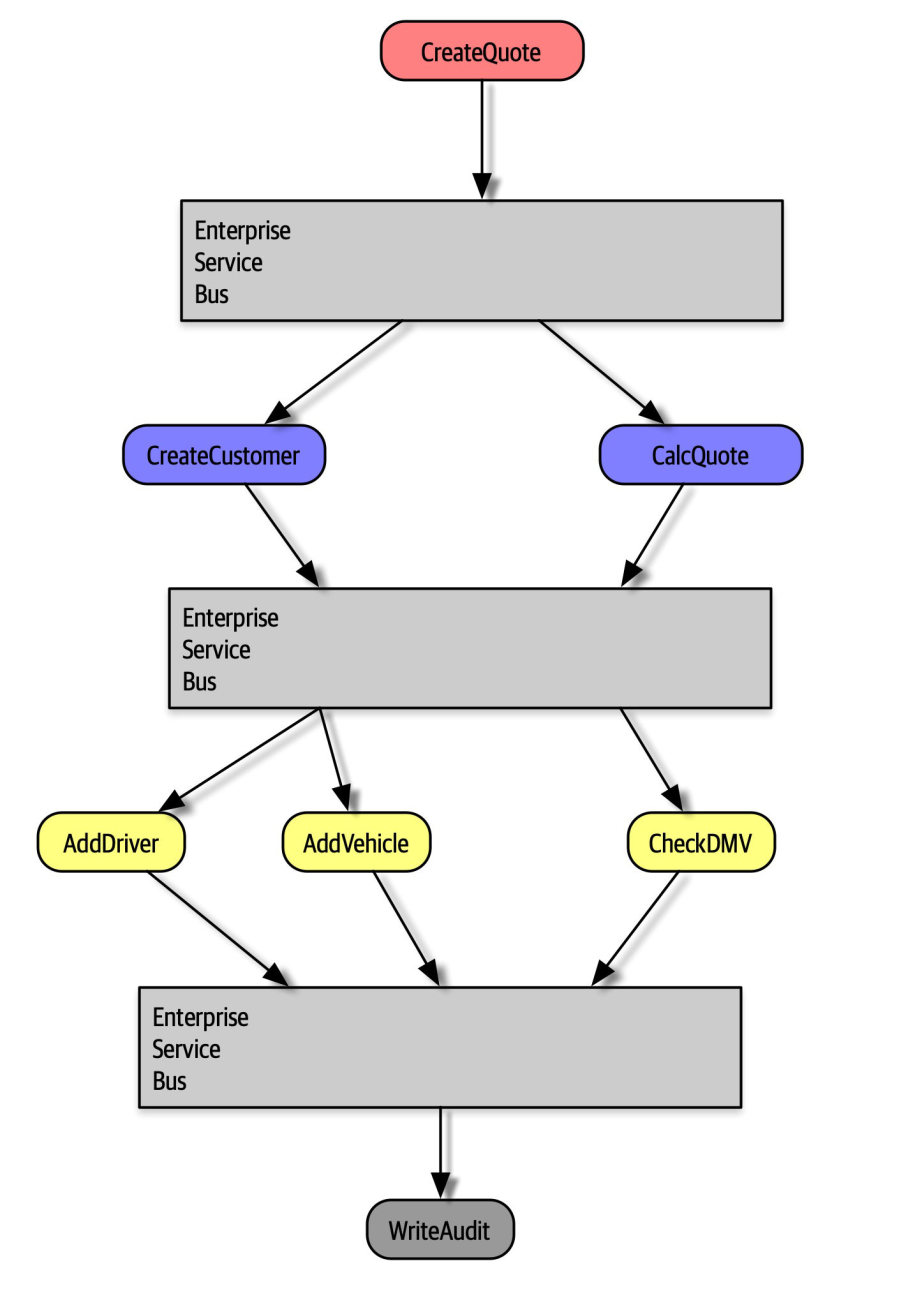
\includegraphics[width=0.5\textwidth]{figura-6-1-flujo-mensajes-soa.png}

        \caption*{Figura 6.1: Flujo de mensajes a través del motor de orquestación. Fuente: Richards y Ford (2020), figura 16-2.}

    \end{figure}

    Ahora bien, la crítica no anula los principios. Los propios autores subrayan que es una idea organizativa que puede tener sentido lógico y aun así obstaculizar el desarrollo, y que estos estilos solo se comprenden en el contexto de su época: la reutilización respondía a un problema real (grandes compañías cansadas de reescribir el mismo software una y otra vez), no a un error de razonamiento (Richards \& Ford, 2020).

    \subsection{Reutilización en Microservicios}

    En la Microservices Architecture cada servicio se ejecuta en su propio proceso, por lo que desacoplarlos en este grado permite una solución simple a un problema común en las arquitecturas que emplean intensivamente infraestructura multiarrendataria para alojar aplicaciones (Richards \& Ford, 2020). Sin embargo, el rendimiento es a menudo el efecto secundario negativo de la naturaleza distribuida de los microservicios, lo que hace que los arquitectos reflexionen cuidadosamente sobre las implicaciones de la granularidad al diseñar el sistema (Richards \& Ford, 2020).

    Cada servicio de la arquitectura de microservicios modela un dominio o un flujo de trabajo; es por eso que cada uno incluye todo lo necesario para operar dentro de la aplicación, incluidas las clases, otros subcomponentes y los esquemas de bases de datos. Los microservicios llevan el concepto de arquitectura particionada por dominios al extremo, al punto de que un arquitecto que construye este estilo de arquitectura prefiere la duplicación al acoplamiento (Richards \& Ford, 2020).

    \subsubsection{Reutilización de lógica de negocio}

    En SOA, la respuesta a un concepto compartido era extraerlo hacia un servicio reutilizable. Richards \& Ford (2020) lo ilustran con una compañía de seguros en la que varias divisiones contienen una noción de Customer. Mencionan que la estrategia adecuada implica extraer las partes de Customer hacia un servicio reutilizable y posibilitar que los servicios originales hagan referencia al servicio de Customer canónico, como se muestra en la Figura 6.2.

    \begin{figure}[H]

        \centering

        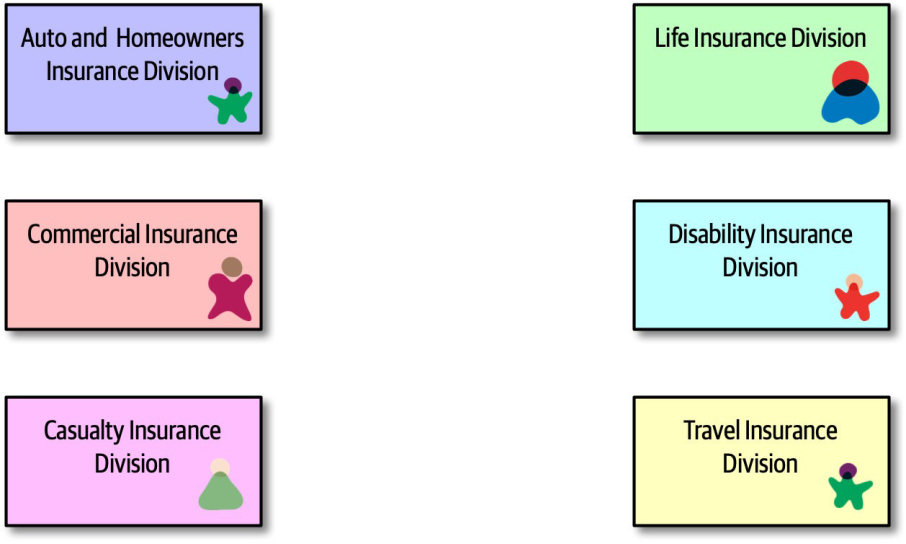
\includegraphics[width=0.5\textwidth]{figura-6-2-oportunidades-reutilizacion.png}

        \caption*{Figura 6.2: Búsqueda de oportunidades de reutilización en la arquitectura orientada a servicios. Fuente: Richards y Ford (2020), figura 16-3.}

    \end{figure}

    Sin embargo, este diseño tenía contrapartidas negativas de las cuales los arquitectos tardaron en darse cuenta. Primero, cuando un equipo construye un sistema principalmente en torno a la reutilización, también incurre en una enorme cantidad de acoplamiento entre componentes, haciendo que cada cambio tuviese un potencial efecto dominó enorme. Ilustrándolo con la compañía de seguros, un cambio en el servicio Customer se propaga en cascada a todos los demás servicios, haciendo arriesgado el cambio (Richards \& Ford, 2020).

    Además, consideremos el caso de los seguros de auto e incapacidad de la Figura 6.3. Para dar soporte a un único servicio Customer, este debe incluir todos los detalles que la organización conoce sobre los clientes. El seguro de auto requiere la licencia de conducir, que es una propiedad de la persona, no del vehículo, por lo que el servicio Customer tendrá que incluir detalles sobre las licencias de conducir con los que la división de seguros de incapacidad no tiene nada que ver. No obstante, el equipo que atiende la incapacidad debe lidiar con la complejidad añadida de una única definición de Customer (Richards \& Ford, 2020).

    \begin{figure}[H]

        \centering

        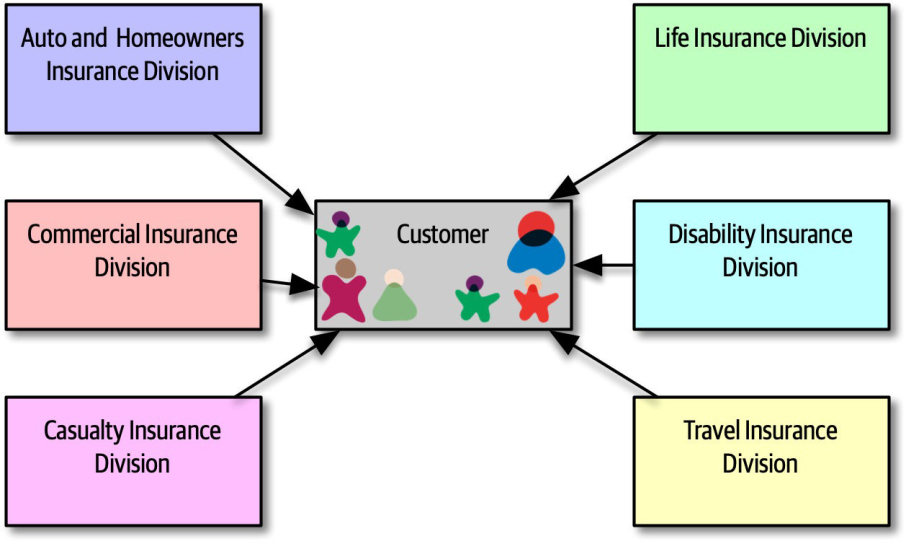
\includegraphics[width=0.5\textwidth]{figura-6-3-representaciones-canonicas.png}

        \caption*{Figura 6.3: Construcción de representaciones canónicas en la arquitectura orientada a servicios. Fuente: Richards y Ford (2020), figura 16-4.}

    \end{figure}

    En los microservicios, la reutilización de la lógica de negocio como la validación de Customer se resuelve de manera opuesta, ya que cada servicio valida lo que necesita dentro de su propio contexto delimitado, con su representación local de Customer. Esta es una consecuencia directa del aislamiento de datos debido a que se trata de evitar todo tipo de acoplamiento, lo cual incluye esquemas compartidos y bases de datos utilizadas como puntos de integración. Cuando los datos se distribuyen a lo largo de la arquitectura ya no es una opción utilizar las bases de datos relacionales para unificar valores dentro de un sistema creando una única fuente de verdad; es por este motivo que los arquitectos deben decidir si manejan este problema identificando un dominio como la fuente de verdad de algún hecho y coordinándose con él para recuperar los valores, o utilizando la replicación de bases de datos o el almacenamiento en caché para distribuir la información. De ahí que los equipos tengan la ventaja, en un sistema altamente desacoplado, de cambiar de opinión y elegir una base de datos (u otra dependencia) más adecuada sin afectar a otros equipos, a los que no se les permite acoplarse a los detalles de la implementación (Richards \& Ford, 2020).

    \subsubsection{Reutilización operativa}

    Las preocupaciones operativas (como la monitorización y el registro) sí se benefician del acoplamiento; sin embargo, los microservicios aplican la reutilización de forma distinta a SOA.

    En la arquitectura orientada a servicios tradicional, una de las filosofías era reutilizar tanta funcionalidad como fuera posible, tanto del dominio como operativa; sin embargo, en los microservicios se opta por separar estas dos preocupaciones (Richards \& Ford, 2020).

    Si una organización permite que cada equipo implemente la monitorización por su cuenta, surgen varias dudas, entre ellas ¿cómo pueden garantizar que cada equipo lo haga? ¿Y cómo manejan preocupaciones como las actualizaciones? ¿Se convierte en responsabilidad de cada equipo gestionar la actualización a la nueva versión de la herramienta de monitorización, y cuánto tiempo llevará eso? La solución a esto es el patrón sidecar, ilustrado en la figura 6.4 (Richards \& Ford, 2020).

    \begin{figure}[H]

        \centering

        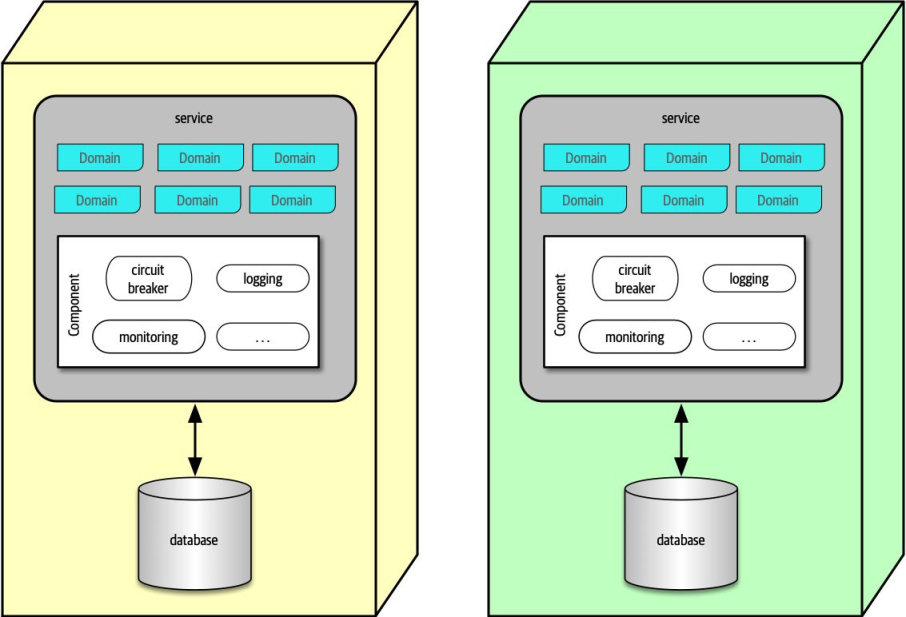
\includegraphics[width=0.5\textwidth]{figura-6-4-sidecar.png}

        \caption*{Figura 6.4: El patrón sidecar en los microservicios. Fuente: Richards y Ford (2020), figura 17-2.}

    \end{figure}

    Las preocupaciones operativas comunes aparecen dentro de cada servicio como un componente separado, que puede ser propiedad de equipos individuales o de un equipo de infraestructura compartida, de modo que, al actualizar el sidecar, cada microservicio recibe esa nueva funcionalidad. Los componentes sidecar comunes se conectan para formar una interfaz operativa consistente en todos los microservicios (Figura 6.5) (Richards \& Ford, 2020).

    \begin{figure}[H]

        \centering

        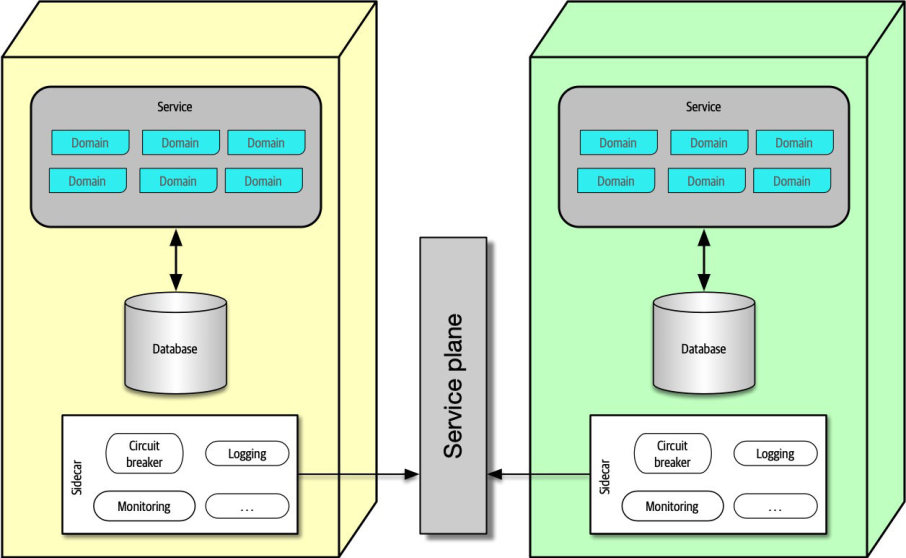
\includegraphics[width=0.5\textwidth]{figura-6-5-malla-servicios.png}

        \caption*{Figura 6.5: El plano de servicios conecta los sidecars en una malla de servicios. Fuente: Richards y Ford (2020), figura 17-3.}

    \end{figure}

    Cada sidecar se conecta al plano de servicios, que forma la interfaz consistente hacia cada servicio. Cada servicio forma un nodo en la malla general (Figura 6.6) y la malla de servicios forma una consola que permite a los equipos controlar globalmente el acoplamiento operativo, como los niveles de monitorización, el registro y otras preocupaciones operativas transversales (Richards \& Ford, 2020).

    \begin{figure}[H]

        \centering

        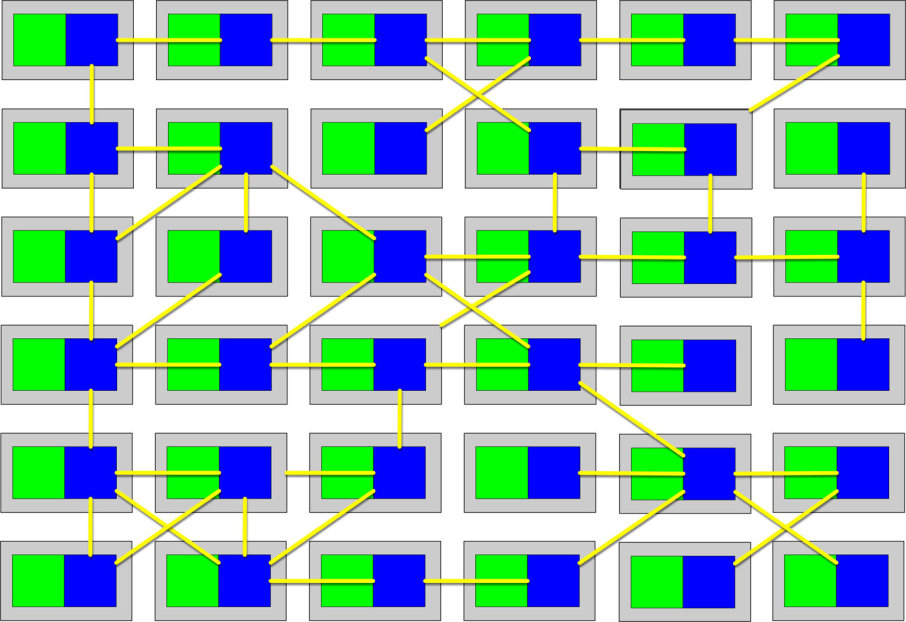
\includegraphics[width=0.5\textwidth]{figura-6-6-vista-holistica.png}

        \caption*{Figura 6.6: La malla de servicios forma una vista holística del aspecto operativo de los microservicios. Fuente: Richards y Ford (2020), figura 17-4.}

    \end{figure}

    \subsection{¿Cuándo conviene todavía un enfoque de orquestación?}

    La Primera Ley de la Arquitectura de Software establece que todo en el software es un trade-off, incluyendo cómo los arquitectos crean los componentes en una arquitectura, de ahí que ninguna alternativa sea perfecta. La coreografía preserva la filosofía de alto desacoplamiento; sin embargo, problemas comunes como el manejo de errores y la coordinación se vuelven más complejos en entornos coreografiados (Richards \& Ford, 2020). El punto débil del estilo sin mediador está documentado en la topología broker de la arquitectura dirigida por eventos, al plantear que el manejo de errores es un gran desafío con esa topología, ya que, al no existir un mediador que supervise o controle la transacción de negocio, si ocurre un fallo, nadie en el sistema se entera de esa caída, provocando que el proceso de negocio se atore y no pueda avanzar sin algún tipo de intervención automatizada o manual, además de que los demás procesos siguen avanzando sin reparar en el error (Richards \& Ford, 2020).

    Cuando un mismo flujo de negocio necesita combinar datos o acciones de varios servicios, como el ejemplo de la lista de deseos donde el servicio \texttt{CustomerWishList} debe llamar a \texttt{CustomerDemographics} para completar la respuesta (figura 6.7); si un arquitecto necesita coordinar a través de varios servicios, tiene la opción de crear su propio mediador localizado: un servicio cuya única responsabilidad es coordinar la llamada e integrar el resultado (figura 6.8) (Richards \& Ford, 2020). Además, la alternativa de no hacerlo es peor ya que, sin mediador, el propio servicio de dominio asume la coordinación y aparece el patrón de controlador frontal, donde un servicio supuestamente coreografiado se convierte en un mediador más complejo para algún problema, con la desventaja de que se le añade complejidad a un servicio (Figura 6.9) (Richards \& Ford, 2020).

    \begin{figure}[H]

        \centering

        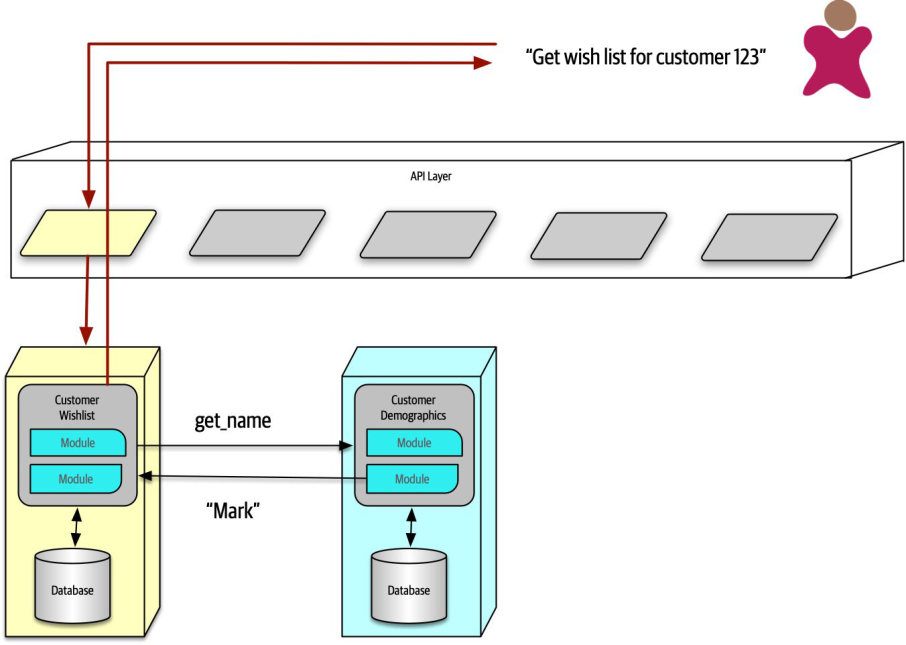
\includegraphics[width=0.5\textwidth]{figura-6-7-coreografia.png}

        \caption*{Figura 6.7: Uso de la coreografía en los microservicios para gestionar la coordinación. Fuente: Richards y Ford (2020), figura 17-7.}

    \end{figure}

    \begin{figure}[H]

        \centering

        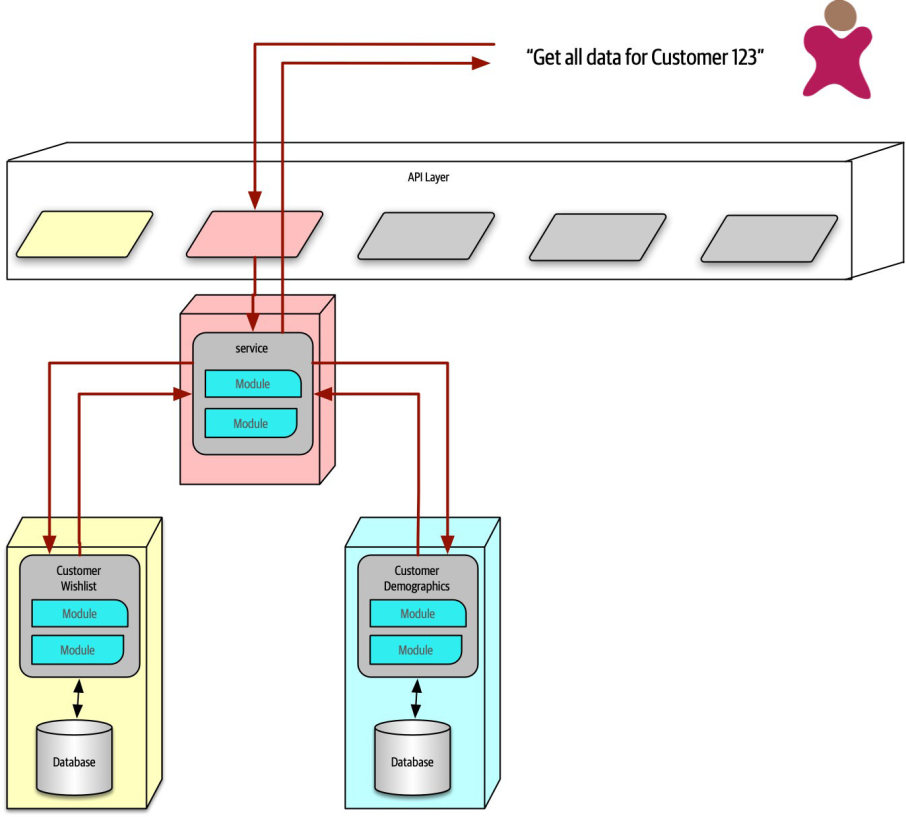
\includegraphics[width=0.5\textwidth]{figura-6-8-orquestacion.png}

        \caption*{Figura 6.8: Uso de la orquestación en los microservicios. Fuente: Richards y Ford (2020), figura 17-8.}

    \end{figure}

    \begin{figure}[H]

        \centering

        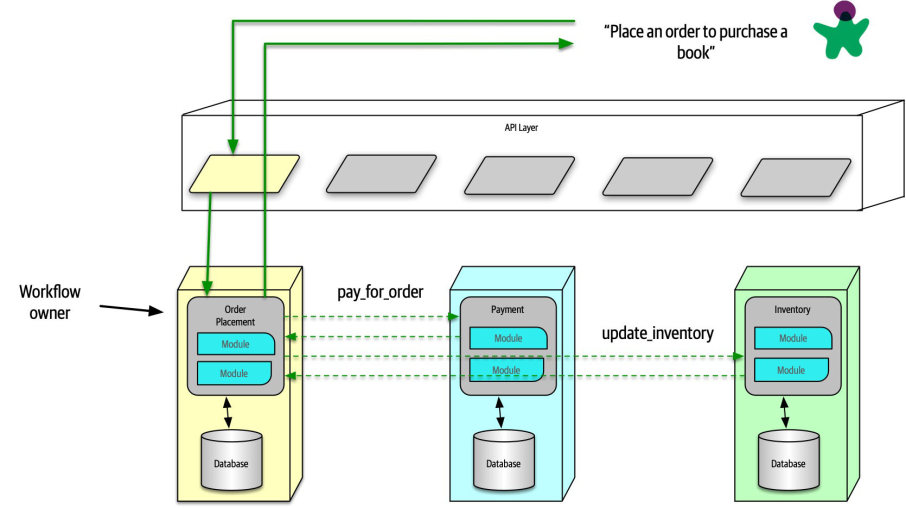
\includegraphics[width=0.5\textwidth]{figura-6-9-coreografia-compleja.png}

        \caption*{Figura 6.9: Uso de la coreografía para un proceso de negocio complejo. Fuente: Richards y Ford (2020), figura 17-9.}

    \end{figure}

    Sin embargo, como bien señalan Richards \& Ford (2020), un arquitecto puede optar por usar la orquestación para procesos de negocio complejos (Figura 6.10) porque, si bien crea acoplamiento entre los servicios, posibilita concentrar la coordinación en un único servicio, dejando a los demás menos afectados. A menudo, los flujos de trabajo del dominio están inherentemente acoplados y el trabajo del arquitecto supone encontrar la mejor manera de representar el acoplamiento en cuestión de forma que se apoyen tanto los objetivos del dominio como los arquitectónicos.

    \begin{figure}[H]

        \centering

        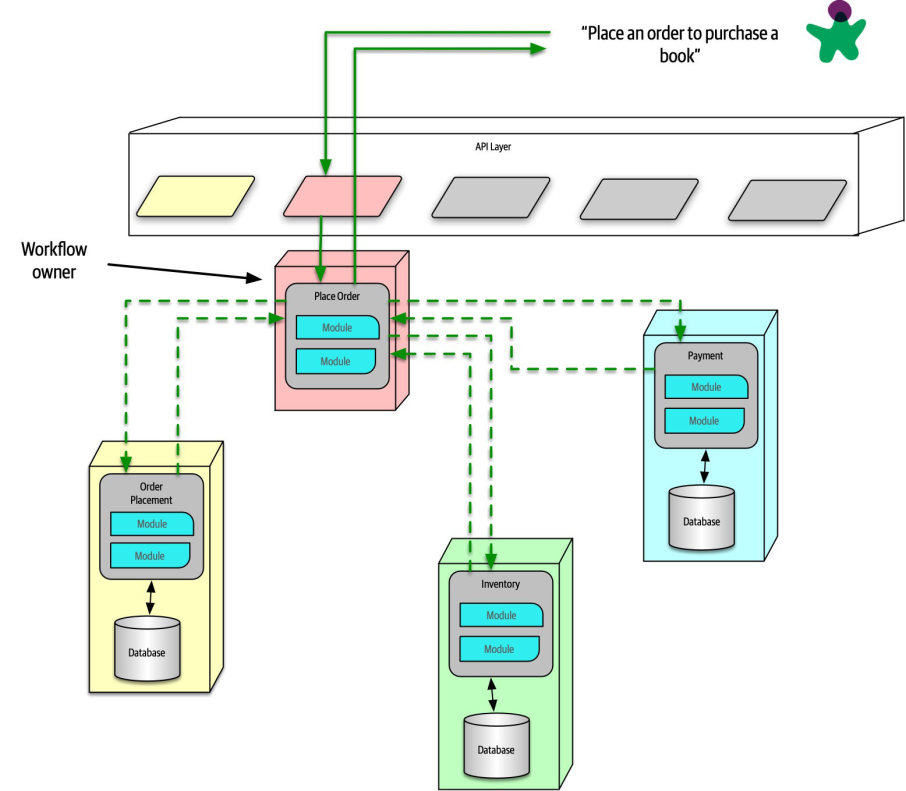
\includegraphics[width=0.5\textwidth]{figura-6-10-orquestacion-compleja.png}

        \caption*{Figura 6.10: Uso de la orquestación para un proceso de negocio complejo. Fuente: Richards y Ford (2020), figura 17-10.}

    \end{figure}

    Dado que el principio de los microservicios es el desacoplamiento y construir transacciones a través de los límites de los servicios constituye una violación del mismo, los arquitectos recomiendan evitarlas y, en su lugar, corregir la granularidad. No obstante, las excepciones siempre existen. Para ilustrarlo, Richards \& Ford (2020) ponen como ejemplo una situación en la que dos servicios diferentes necesiten características arquitectónicas muy distintas, lo que requiere límites de servicio diferenciados, y a pesar de ello necesiten coordinación transaccional. Plantean como respuesta un patrón de saga: un servicio actúa como mediador, llama a cada parte de la transacción, registra el éxito o el fracaso, coordina los resultados y, ante un fallo, envía una solicitud a todas las partes de la transacción que fueron exitosas y les pide que deshagan la solicitud anterior, es decir, gestiona las transacciones compensatorias (figuras 6.11 y 6.12).

    \begin{figure}[H]

        \centering

        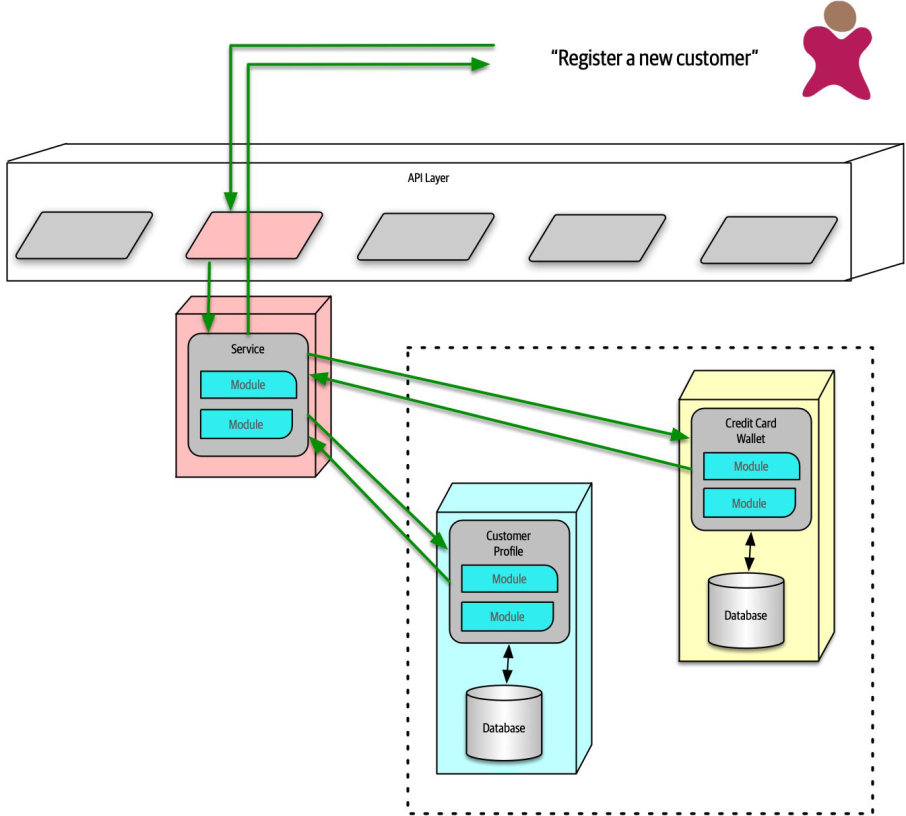
\includegraphics[width=0.5\textwidth]{figura-6-11-saga.png}

        \caption*{Figura 6.11: El patrón de saga en la arquitectura de microservicios. Fuente: Richards y Ford (2020), figura 17-11.}

    \end{figure}

    \begin{figure}[H]

        \centering

        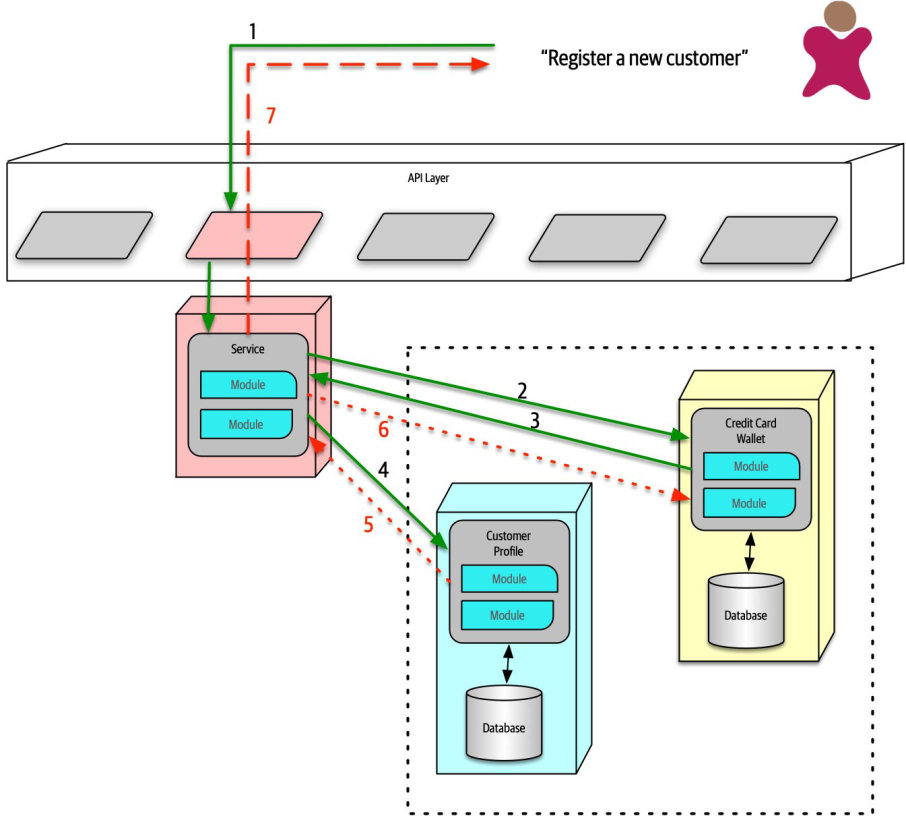
\includegraphics[width=0.5\textwidth]{figura-6-12-transacciones-compensatorias.png}

        \caption*{Figura 6.12: Transacciones compensatorias del patrón de saga para condiciones de error. Fuente: Richards y Ford (2020), figura 17-12.}

    \end{figure}

    El capítulo 9 de Software Architecture: The Hard Parts muestra la misma idea en su forma más útil: se emplea un servicio de orquestación dedicado para la petición de negocio, que libera a los servicios de dominio de la gestión transaccional y favorece la consistencia de datos sobre la capacidad de respuesta, asumiendo a cambio un manejo de errores complejo donde el orquestador debe decidir si reintenta, compensa o escala el problema (figuras 6.13 y 6.14) (Ford, Richards, Sadalage \& Dehghani, 2021).

    \begin{figure}[H]

        \centering

        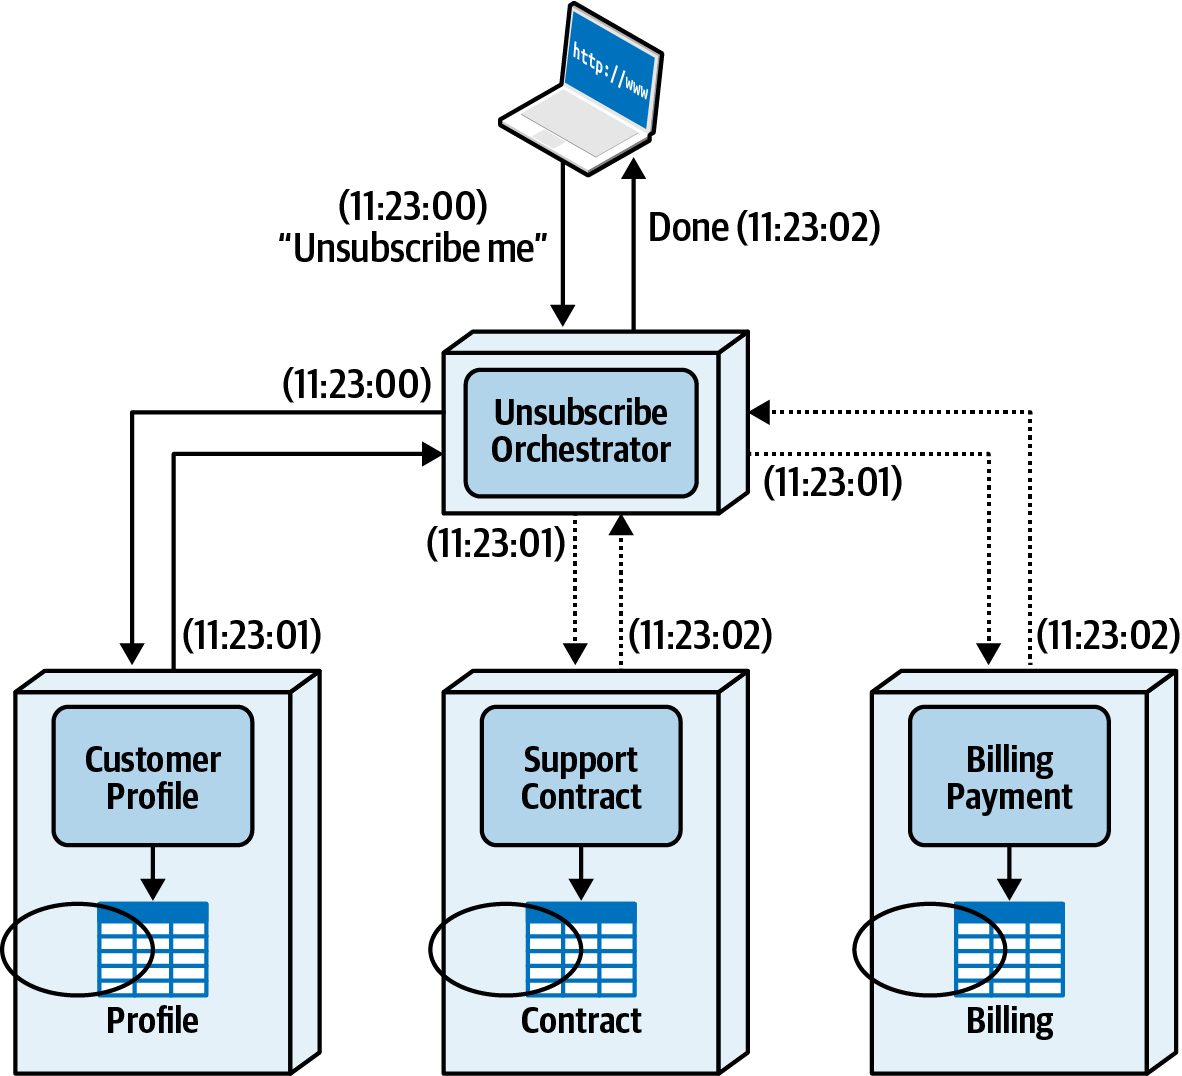
\includegraphics[width=0.5\textwidth]{figura-6-13-servicio-orquestacion-dedicado.png}

        \caption*{Figura 6.13: Un servicio de orquestación dedicado asume el rol de orquestador de la transacción. Fuente: Ford, Richards, Sadalage y Dehghani (2021), figura 9-18.}

    \end{figure}

    \begin{figure}[H]

        \centering

        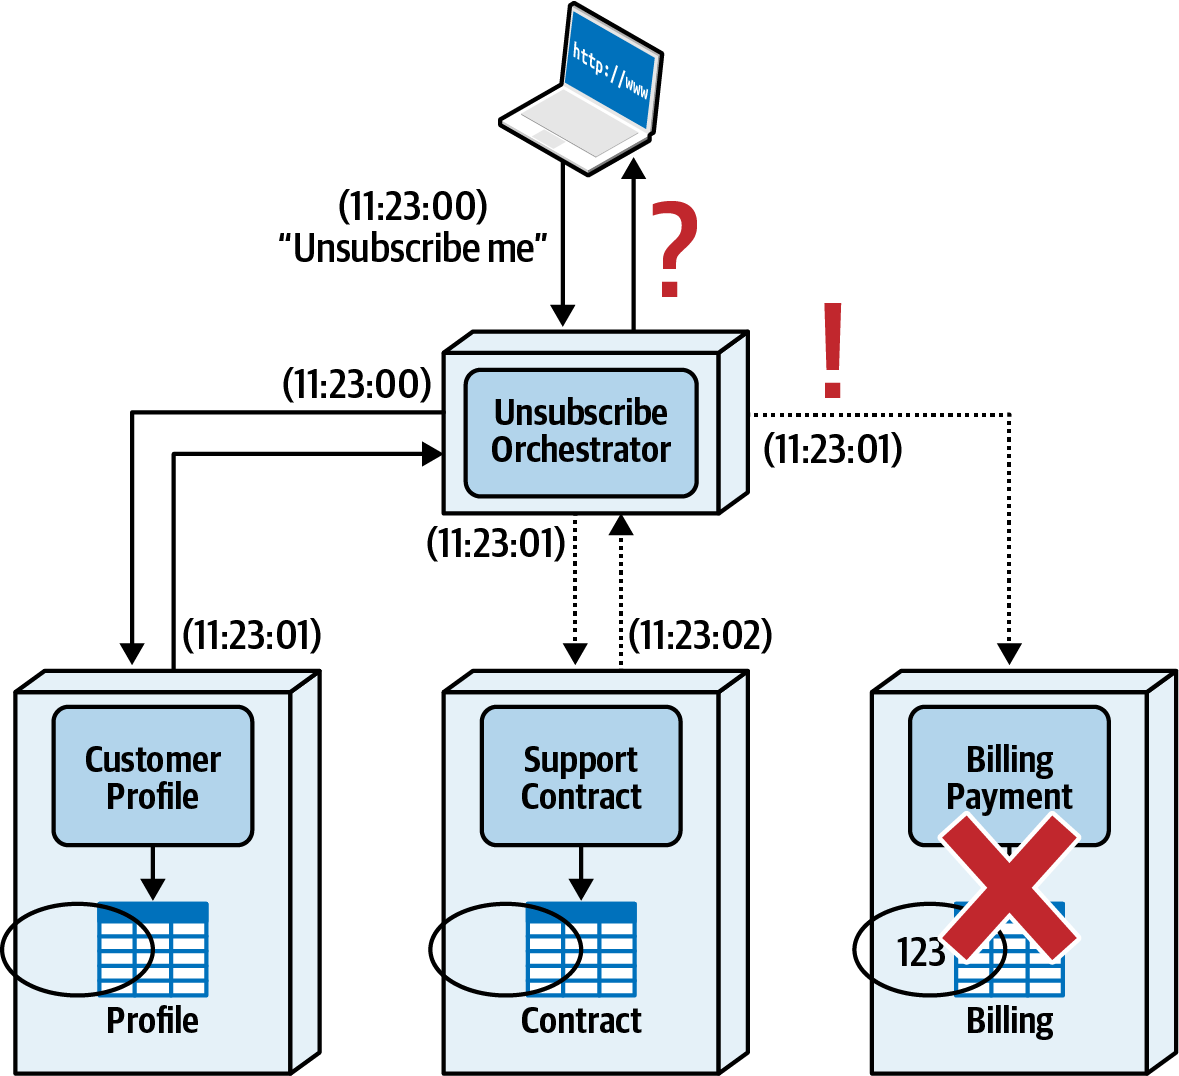
\includegraphics[width=0.5\textwidth]{figura-6-14-errores-patron-orquestado.png}

        \caption*{Figura 6.14: Las condiciones de error son muy difíciles de abordar cuando se utiliza el patrón basado en peticiones orquestadas. Fuente: Ford, Richards, Sadalage y Dehghani (2021), figura 9-19.}

    \end{figure}

    La cantidad de orquestación conveniente depende de la complejidad del flujo: para eventos que requieren un manejo de errores y una orquestación simple, un mediador como Apache Camel, Mule ESB o Spring Integration suele bastar; si el flujo de trabajo del evento requiere mucho procesamiento condicional y múltiples rutas dinámicas con directivas complejas de manejo de errores, entonces un mediador como Apache ODE o el Oracle Process Manager sería una buena elección; y para flujos de eventos que requieren transacciones de larga duración con intervención humana, un motor BPM como jBPM, como en el ejemplo de una operación bursátil que se detiene para esperar la aprobación manual de un operador senior (Richards \& Ford, 2020). Los autores advierten de la importancia de conocer los tipos de eventos que se procesarán a través del mediador para hacer la elección correcta, pues elegir una herramienta por debajo del problema sería extremadamente difícil de escribir y mantener, mientras que escoger una que esté por encima tomaría meses de esfuerzo desperdiciado.

    \subsection{Ejemplo de flujo complejo con orquestación explícita}

    Para el flujo complejo que se beneficia de la orquestación explícita usamos el ejemplo del capítulo 14 (Richards \& Ford, 2020): el procesamiento de un pedido de compra. Lo separaremos en pasos:

    \begin{enumerate}

        \item Realizar el pedido: Crear el pedido.

        \item Procesar el pedido: Enviar un correo al cliente informándole que el pedido ha sido realizado, aplicar pago y decrementar inventario.

        \item Completar el pedido: Preparar y empaquetar el pedido, ordenar más existencias al proveedor, de ser necesario.

        \item Enviar orden: Enviar un correo al cliente informándole que su pedido está listo para ser enviado, enviar el pedido al cliente.

        \item Notificar al cliente: Enviar un email al cliente informándole que el pedido ha sido enviado.

    \end{enumerate}

    Una vez que el evento de inicio (\texttt{PlaceOrder}) ha sido recibido, el mediador de \textbf{Customer} genera un evento de procesamiento \texttt{create-order} y envía este mensaje a la cola de colocación de pedidos (\texttt{order-placement-queue}) (ver Figura 6.15). El procesador de eventos \textbf{OrderPlacement} acepta este evento, valida y crea el pedido y devuelve al mediador un acuse de recibo junto con el ID del pedido. En este punto, el mediador podría enviar ese ID de pedido de vuelta al cliente, indicando que el pedido quedó realizado, o podría continuar hasta que se completen todos los pasos según especifiquen las reglas de negocio.

    \begin{figure}[H]

        \centering

        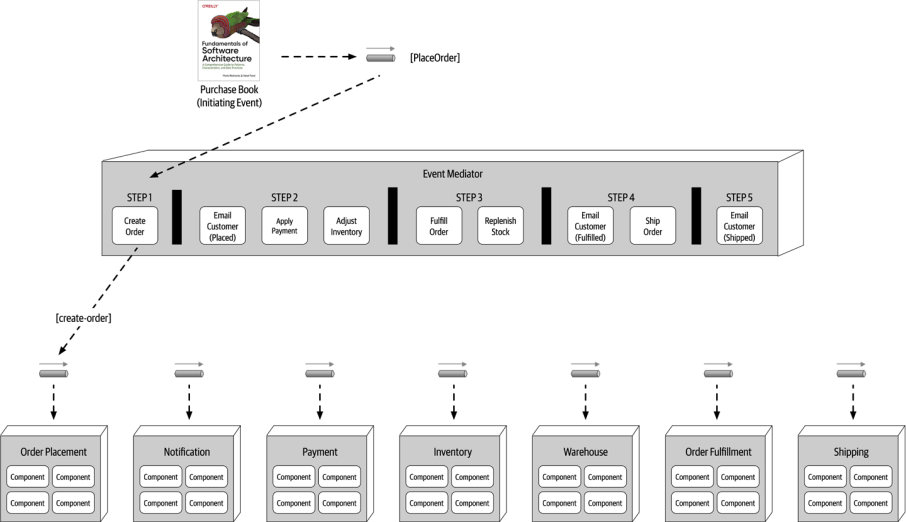
\includegraphics[width=0.75\textwidth]{figura-6-15-ejemplo-mediador-paso1.png}

        \caption*{Figura 6.15: Paso 1 del ejemplo del mediador. Fuente: Richards y Ford (2020), figura 14-8.}

    \end{figure}

    Luego el mediador genera tres mensajes al mismo tiempo: \texttt{email-customer}, \texttt{apply-payment} y \texttt{adjust-inventory}. Estos eventos de procesamiento se envían todos a sus respectivas colas. Los tres procesadores de eventos reciben estos mensajes, realizan sus respectivas tareas y notifican al mediador que el procesamiento se ha completado. El mediador espera a recibir el acuse de recibo de los tres procesos en paralelo antes de pasar al paso siguiente (Figura 6.16).

    \begin{figure}[H]

        \centering

        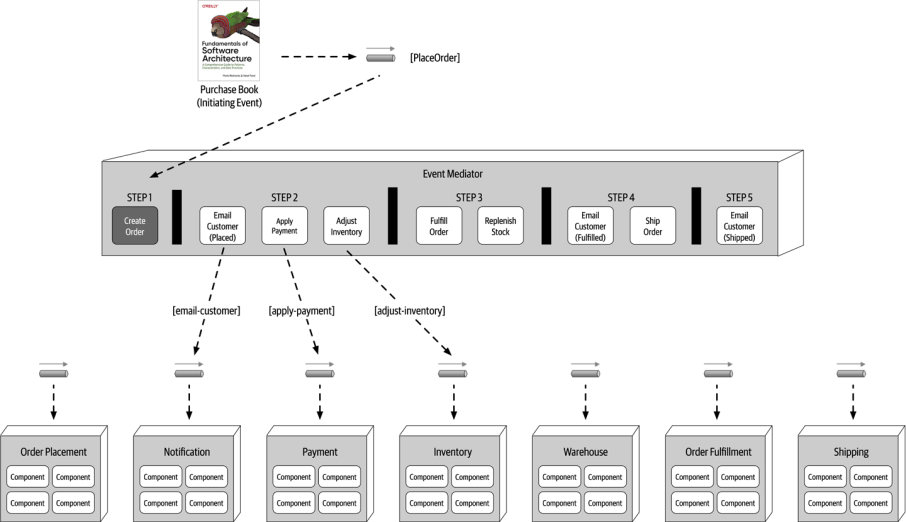
\includegraphics[width=0.75\textwidth]{figura-6-16-ejemplo-mediador-paso2.png}

        \caption*{Figura 6.16: Paso 2 del ejemplo del mediador. Fuente: Richards y Ford (2020), figura 14-9.}

    \end{figure}

    Una vez recibidos, se puede pasar al paso 3 para cumplir el pedido (ver figura 6.17). En este paso, los dos eventos \texttt{fulfill-order} y \texttt{order-stock} también pueden ocurrir simultáneamente. Los procesadores de eventos \textbf{OrderFulfillment} y \textbf{Warehouse} aceptan esos eventos, realizan su trabajo y devuelven un acuse de recibo al mediador.

    \begin{figure}[H]

        \centering

        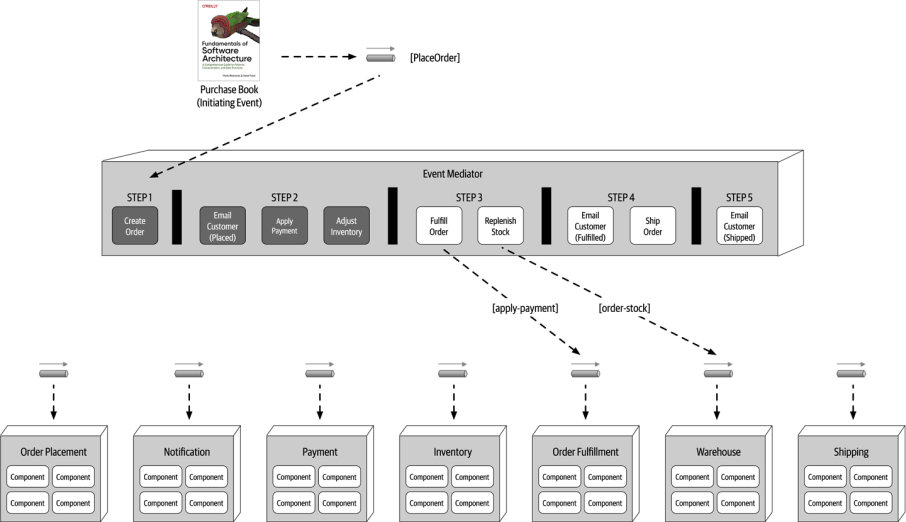
\includegraphics[width=0.75\textwidth]{figura-6-17-ejemplo-mediador-paso3.png}

        \caption*{Figura 6.17: Paso 3 del ejemplo del mediador. Fuente: Richards y Ford (2020), figura 14-10.}

    \end{figure}

    Es solo cuando se completan estos eventos que el mediador pasa al paso 4 (ver figura 6.18) para enviar el pedido. Este paso genera otro evento de procesamiento \texttt{email-customer} con información específica sobre qué hacer (notificar al cliente que el pedido está listo para despacharse), así como un evento \texttt{ship-order}.

    \begin{figure}[H]

        \centering

        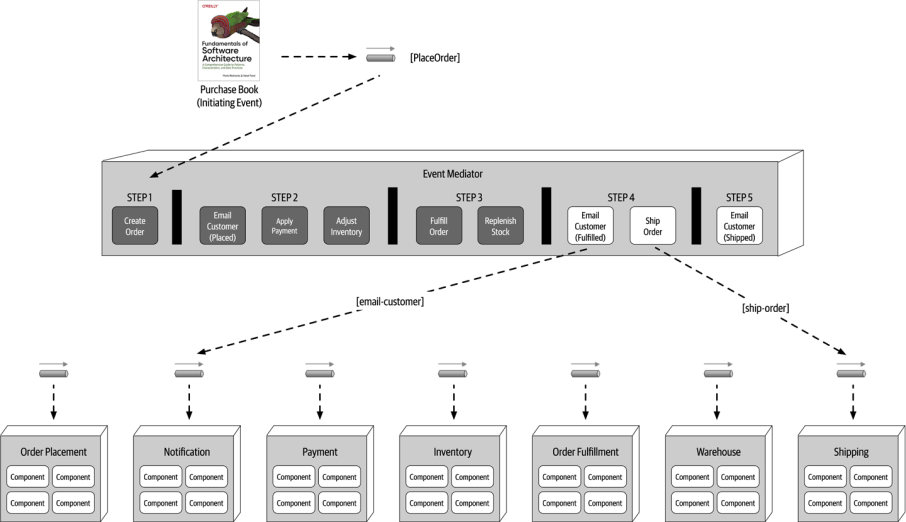
\includegraphics[width=0.75\textwidth]{figura-6-18-ejemplo-mediador-paso4.png}

        \caption*{Figura 6.18: Paso 4 del ejemplo del mediador. Fuente: Richards y Ford (2020), figura 14-11.}

    \end{figure}

    Para finalizar, el mediador pasa al último paso (ver figura 6.19) y genera otro evento \texttt{email-\allowbreak customer}, esta vez para notificar al cliente que el pedido ha sido despachado. En este punto el flujo de trabajo termina, el mediador marca el flujo de eventos de inicio como completo y elimina todo el estado asociado con el evento de inicio.

    \begin{figure}[H]

        \centering

        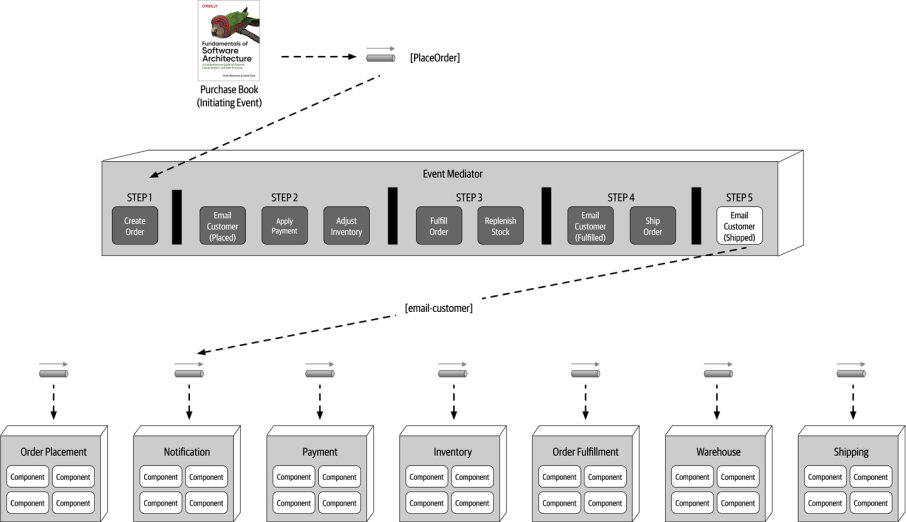
\includegraphics[width=0.75\textwidth]{figura-6-19-ejemplo-mediador-paso5.png}

        \caption*{Figura 6.19: Paso 5 del ejemplo del mediador. Fuente: Richards y Ford (2020), figura 14-12.}

    \end{figure}

    El componente mediador tiene conocimiento y control del flujo de trabajo, por lo tanto, puede mantener el estado del evento y gestionar el manejo de errores, la capacidad de recuperación y de reinicio. Los autores ponen el siguiente ejemplo: supóngase que el pago no se aplicó debido a que la tarjeta de crédito estaba vencida. En este caso, el mediador recibe esta condición de error y, sabiendo que el pedido no puede cumplirse hasta que el pago sea aplicado, detiene el flujo de trabajo y registra el estado de la petición en su propio almacén de datos persistente. Una vez que el pago finalmente se aplica, el flujo de trabajo puede reiniciarse desde donde se quedó.

    \section{Bibliografía}

    \begin{itemize}

        \item Richards, M., \& Ford, N. (2020). \textit{Fundamentals of Software Architecture: An Engineering Approach}. O'Reilly Media.

        \item Ford, N., Richards, M., Sadalage, P., \& Dehghani, Z. (2021). \textit{Software Architecture: The Hard Parts}. O'Reilly Media.

    \end{itemize}

    \newpage
    \section{Declaración de uso de IA}

    En la elaboración de este documento se empleó asistencia de herramientas de inteligencia artificial para las siguientes tareas:

    \begin{itemize}
        \item La traducción de los capítulos de los libros que sirven de base bibliográfica al trabajo.
        \item La conversión del documento Word al formato LaTeX.
        \item La revisión de la ortografía del texto.
    \end{itemize}

    Todo el contenido generado fue revisado, verificado y adaptado por el equipo, quien asume la responsabilidad final del documento.

\end{document}
